%%%%%%%%%%%%%%%%%%%%%%%%%%%%%%%%%%%%%%%%%%%%%%%%%%%%%%%%%%%%%%%%%%%%%%%%%%%%
% Nick Waters's super awesome template for bioRxiv and suppl submissions
% In memory of Henry, Hermione, and Angus.
% May there be many tasty snails in pufferfish heaven
%%%%%%%%%%%%%%%%%%%%%%%%%%%%%%%%%%%%%%%%%%%%%%%%%%%%%%%%%%%%%%%%%%%%%%%%%%%%
\documentclass[10pt]{article}

\usepackage{geometry}
\geometry{marginparwidth=1cm,a4paper,verbose,tmargin=1.5cm,bmargin=1.5cm,lmargin=1.5cm,rmargin=1.5cm,headheight=0cm,headsep=0cm,footskip=0cm}
\usepackage{cite}
\usepackage{float}  % for forcing figures to stay put
\usepackage{hyperref} % make the references clickable
\setlength\parindent{0pt} % set indent to zero
\setlength{\parskip}{1.2em} % give a bit of space between paragraphs

\bibliographystyle{plain} % citation and bib style
\usepackage{grffile} %for underscores in file names
\usepackage[ruled]{algorithm2e} % for typesetting the riboSeed algorithm
\setlength{\algotitleheightrule}{0pt}
\usepackage{lineno, color} % controls line numbering
\modulolinenumbers[5]  % number every 5th line
% format our line numbers, cause no one likes boring numbers
\renewcommand\linenumberfont{\normalfont\tiny\color{blue}}
\usepackage{booktabs}  % less yucky tables
% nice little thing for table spacing (thanks Markus Püschel)
\newcommand{\ra}[1]{\renewcommand{\arraystretch}{#1}}
\usepackage{multirow} % for some pretty tables with merged cells
\usepackage[table,xcdraw]{xcolor} % for cool table cell colors
% my lined-off abstract
\newenvironment{myabstract}{%
\begin{quote} \baselineskip14pt \rule{.89\textwidth}{1.5pt} \vskip .1cm}
{ \vskip -.10cm \rule{.89\textwidth}{1.5pt} \end{quote}}

% supplementary (essentialy just resets numbering)
\newcommand{\beginsupplement}{%
  \setcounter{table}{0}
  \renewcommand{\thetable}{S\arabic{table}}%
  \setcounter{figure}{0}
  \renewcommand{\thefigure}{S\arabic{figure}}%
}
% pretty thought break
\def \thoughtbr {\begin{center}\noindent\rule{.4\textwidth}{0.4pt}  {\raisebox{-.5ex}{$\sim$}}  \rule{.4\textwidth}{0.4pt}\end{center}}

% \usepackage{graphicx}
\graphicspath{ {../riboSeed/Waters_et_al_2017/ms/riboFigs/} }  %  set the path to the figures

\usepackage{titlesec} % for adjusting spacing after the section headers
\titlespacing\subsection{0pt}{12pt plus 4pt minus 2pt}{-11pt plus 0pt minus 0pt}
\titlespacing\subsubsection{0pt}{12pt plus 4pt minus 2pt}{-11pt plus 0pt minus 0pt}


%%%%%%%%%%%%%%%%%%%%%%%%%%%%%%%%%%%%%%%%%%%%%%%%%%
% this hack stolen from Stack overflow is a macro to make a \cmmidrule
% for each column.  I added the ".4" spacing to get this to look prettier
%  if you have 5 columns, instead of \midrule, you could use \cmidrules{5}
\makeatletter
\newtoks\MD@cmidrules
\newcommand{\cmidrules}[1]{%
  \noalign{%
    \global\MD@cmidrules={}%
    \toks@={\cmidrule(l{.3\tabcolsep}r{.3\tabcolsep})}%
    \count@=\z@
    \loop\ifnum\count@<#1\relax
      \advance\count@\@ne
      \edef\MD@temp{\the\toks@{\the\count@-\the\count@}}%
      \global\MD@cmidrules\expandafter{\the\expandafter\MD@cmidrules\MD@temp}%
    \repeat
  }%
  \the\MD@cmidrules
}
\makeatother
%%%%%%%%%%%%%%%%%%%%%%%%%%%%%%%%%%%%%%%%%%%%%%%%%%

%%%%  This allows us to set the table font size up top
\usepackage{etoolbox}
\BeforeBeginEnvironment{tabular}{\begin{center}\footnotesize}
\AfterEndEnvironment{tabular}{\end{center}}
%%%%

\def \coli#1 {\textit{E.~coli~#1~}} %  #lazy
\def \ttilde {\raisebox{-.5ex}\textasciitilde} % fix for ugly cmodern tilde 20160829

%  format captions
\usepackage[%
    font={small},
    labelfont=bf,
    format=hang,
    format=plain,
    margin=0pt,
    width=0.9\textwidth]{caption}
\usepackage[list=true]{subcaption}  % allow for subfigures with captions
\usepackage{amssymb}  % for checkmark symbols
\usepackage{graphicx}  % trim figures
\usepackage{colortbl}  % adjust table colors
\definecolor{lgray}{gray}{.90}  % line grey
\definecolor{tgray}{gray}{.40}  % text grey
\definecolor{egray}{gray}{.01}  % emphasis grey
\usepackage[yyyymmdd,hhmmss]{datetime} % for timestamp

\title{\textbf{Supplementary Data}\\ \fontseries{m}\selectfont riboSeed: leveraging prokaryotic genomic architecture to assemble across ribosomal regions}

\author
{\small Nicholas R. Waters,$^{1,2}$ Florence Abram,$^{1}$ Fiona Brennan,$^{1,3}$ Ashleigh Holmes,$^{4}$ and Leighton Pritchard$^{2\ast}$\\
\\
\normalsize{\textit {$^{1}$Department of Microbiology, School of Natural Sciences, National University of Ireland, Galway, Ireland}}\\
\normalsize{\textit {$^{2}$Information and Computational Sciences, James Hutton Institute, Invergowrie, Dundee DD2 5DA, Scotland}}\\
\normalsize{\textit {$^{3}$Soil and Environmental Microbiology, Environmental Research Centre, Teagasc, Johnstown Castle, Wexford, Ireland}}\\
\normalsize{\textit {$^{4}$Cell and Molecular Sciences, James Hutton Institute, Invergowrie, Dundee DD2 5DA, Scotland}}\\
\\
\footnotesize{$^\ast$To whom correspondence should be addressed: leighton.pritchard@hutton.ac.uk}
}
\date{}

\begin{document}
\baselineskip20pt  % set line spacing; double spacing is 2xfontsize, in this case 11
\maketitle
\vspace*{-1.5cm}
{\begin{center}\footnotesize\date{Compiled: \today ~\currenttime}\end{center}}

\beginsupplement

\SetKwProg{Scan}{riboScan}{ }{end}
\SetKwProg{Select}{riboSelect}{ }{end}
\SetKwProg{Seed}{riboSeed}{ }{end}
\begin{figure}[h]
  \centering
  \begin{minipage}{.6\linewidth}
    \begin{algorithm}[H]
      % \KwData{reference, reads}
      %  % initialization\;
      % \Scan{(reference fastas)}{
      % \For{chromosome in reference}{
      % run Barrnap to find rRNAs\;
      % add locus tags to gff\;
      % convert to genbank\;
      % }
      %   combine genbanks\;
      %   return scannedScaffolds\;
      % }
      %   \hrule
      % % \end{algorithm}
      % % \pagebreak
      % % \begin{algorithm}[H]
      %   \Select{(scannedScaffolds)}{
      %   parse coordinated of rRNAs\;
      %   cluster into operons\;
      %   return grouped\_loci\;
      % }
      %   \hrule
      % \end{algorithm}
      % \pagebreak
      % \begin{algorithm}[H]
      %   \Seed{(scannedScaffolds, grouped\_loci, reads, iters)}{
      %   reference = scannedScaffolds\;
      %   clusters = parse grouped\_loci\;
      %   \For{i in iters}{
      %   map reads to reference\;
      %   \For{cluster in clusters}{
      %   filter and extract reads within clusters and flanking\;
      %   subassemble with SPAdes\;
      %   return pseudocontig\;
      % }
      %   assess subassembly\;
      %   \If {success}{
      %   make fauxgenome from pseudocontigs \;
      %   reference = fauxgenome
      %   continue
      % }
      %   \If{last iteration}{
      %   run SPAdes with pseudocontigs\;
      % }
      % }
      % }
      \Seed{(reference, riboSelect\_clusters, reads, iters, flanking\_width)}{
        ref = reference\;
        clusters = parse riboSelect\_clusters\;
        region = clusters + flanking\_width\;
        \For{i in iters}{
          map reads to ref\;
          \For{cluster in clusters}{
            filter and extract reads region\;
            subassemble\;
            return pseudocontig\;
          }
          assess subassembly\;
          \If {success}{
            make pseudogenome from pseudocontigs \;
            ref = pseudogenome \;
          }
        }
        run assembler with reads and pseudocontigs\;
      }
    \end{algorithm}
  \end{minipage}
  \caption{Pseudocode of riboSeed algorithm}
  \label{fig:algo}
\end{figure}
%%%%%%%%%%%%%%%%%%%%%%%%%%%%%%%%%%%%%%%%%%%%%%%%%%%% 5


\begin{figure}[H]
    \centering
    \hspace*{0cm}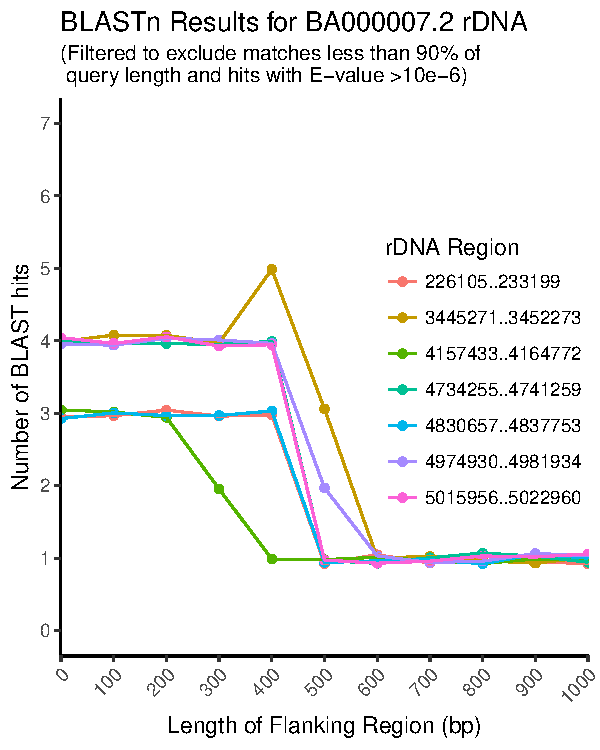
\includegraphics[width=.5\textwidth]{grouped_sakai_BLAST_results}
    \caption{BLASTn was used to perform \textit{in silico} DNA-DNA hybridization of all rDNA regions from \textit{E. coli Sakai} with variable flanking lengths. The number of hits is a proxy for occurrences in the genome; increasing the flanking length increases the specificity. (Points are jittered to aide visibility for overlapping values.)}
    \label{fig:blast}
  \end{figure}

\begin{figure}[H]
    \centering
    \hspace*{0cm}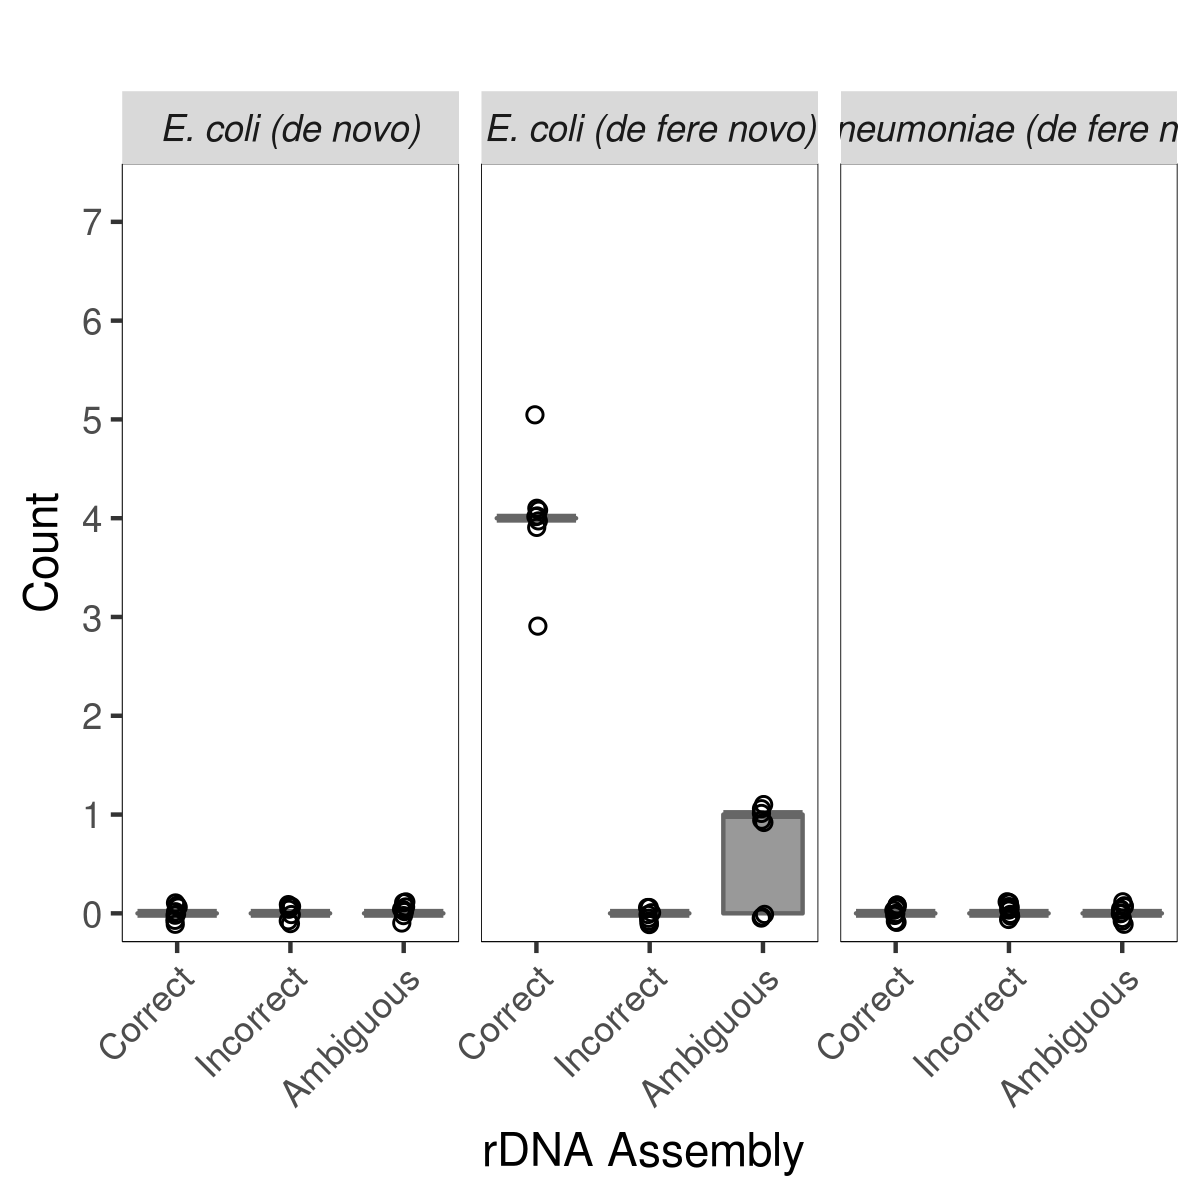
\includegraphics[width=.60\textwidth]{simulated_genome}
    \caption{Assembly of artificial genome. \textit{De fere novo} results in closure of 3-5 rDNAs with the correct reference; only 1-2 rDNAs are correctly assembled using \textit{K. pneumoniae}.  No rDNAs are assembled with \textit{de novo} assembly. Scored with riboScore.py. N=8.}
    \label{fig:simgenome}
\end{figure}


\begin{figure}[H]
  \centering
  \begin{subfigure}[b]{.45\textwidth}
    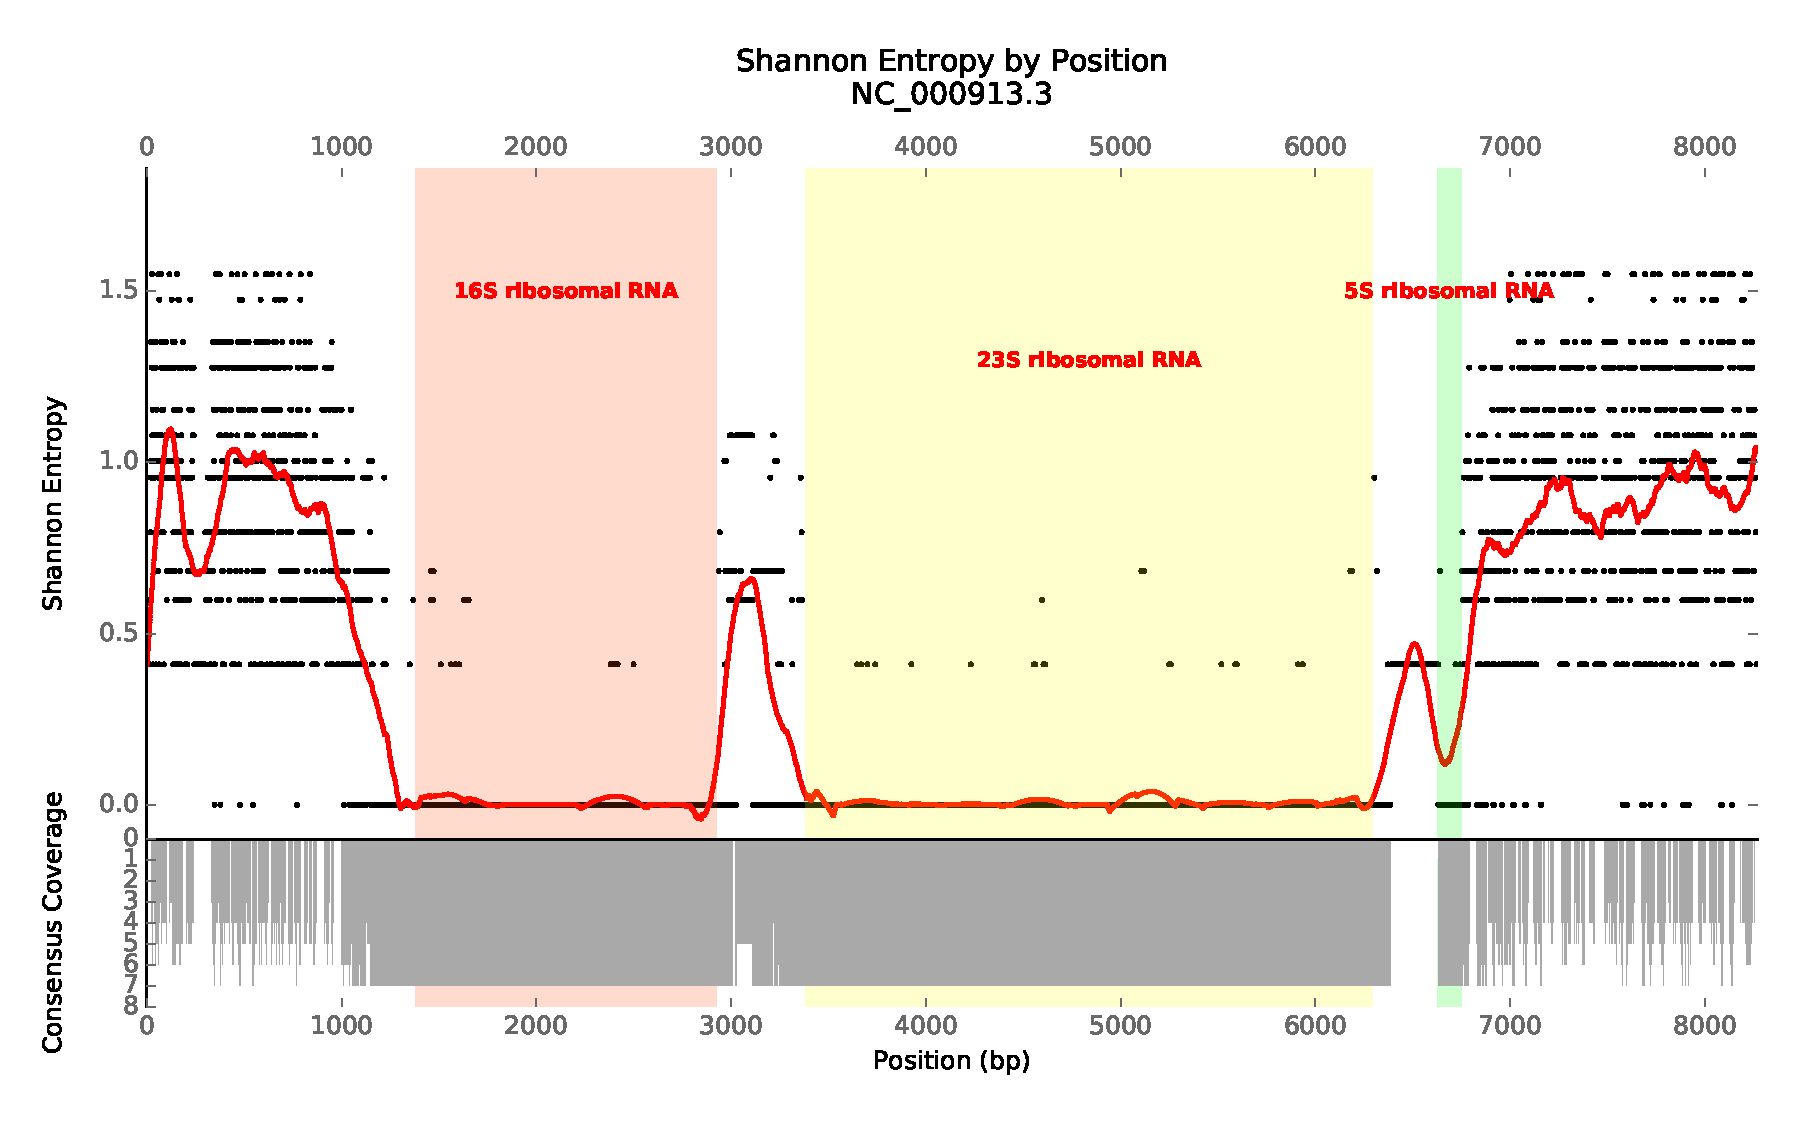
\includegraphics[width=0.95\textwidth]{gage_entropy_figures/NC_000913.3_entropy_plot}
    \caption{\textit{E. coli MG1655} (NC\_000913.3)}
    \label{fig:ent_coli}
  \end{subfigure}
  \begin{subfigure}[b]{.45\textwidth}
    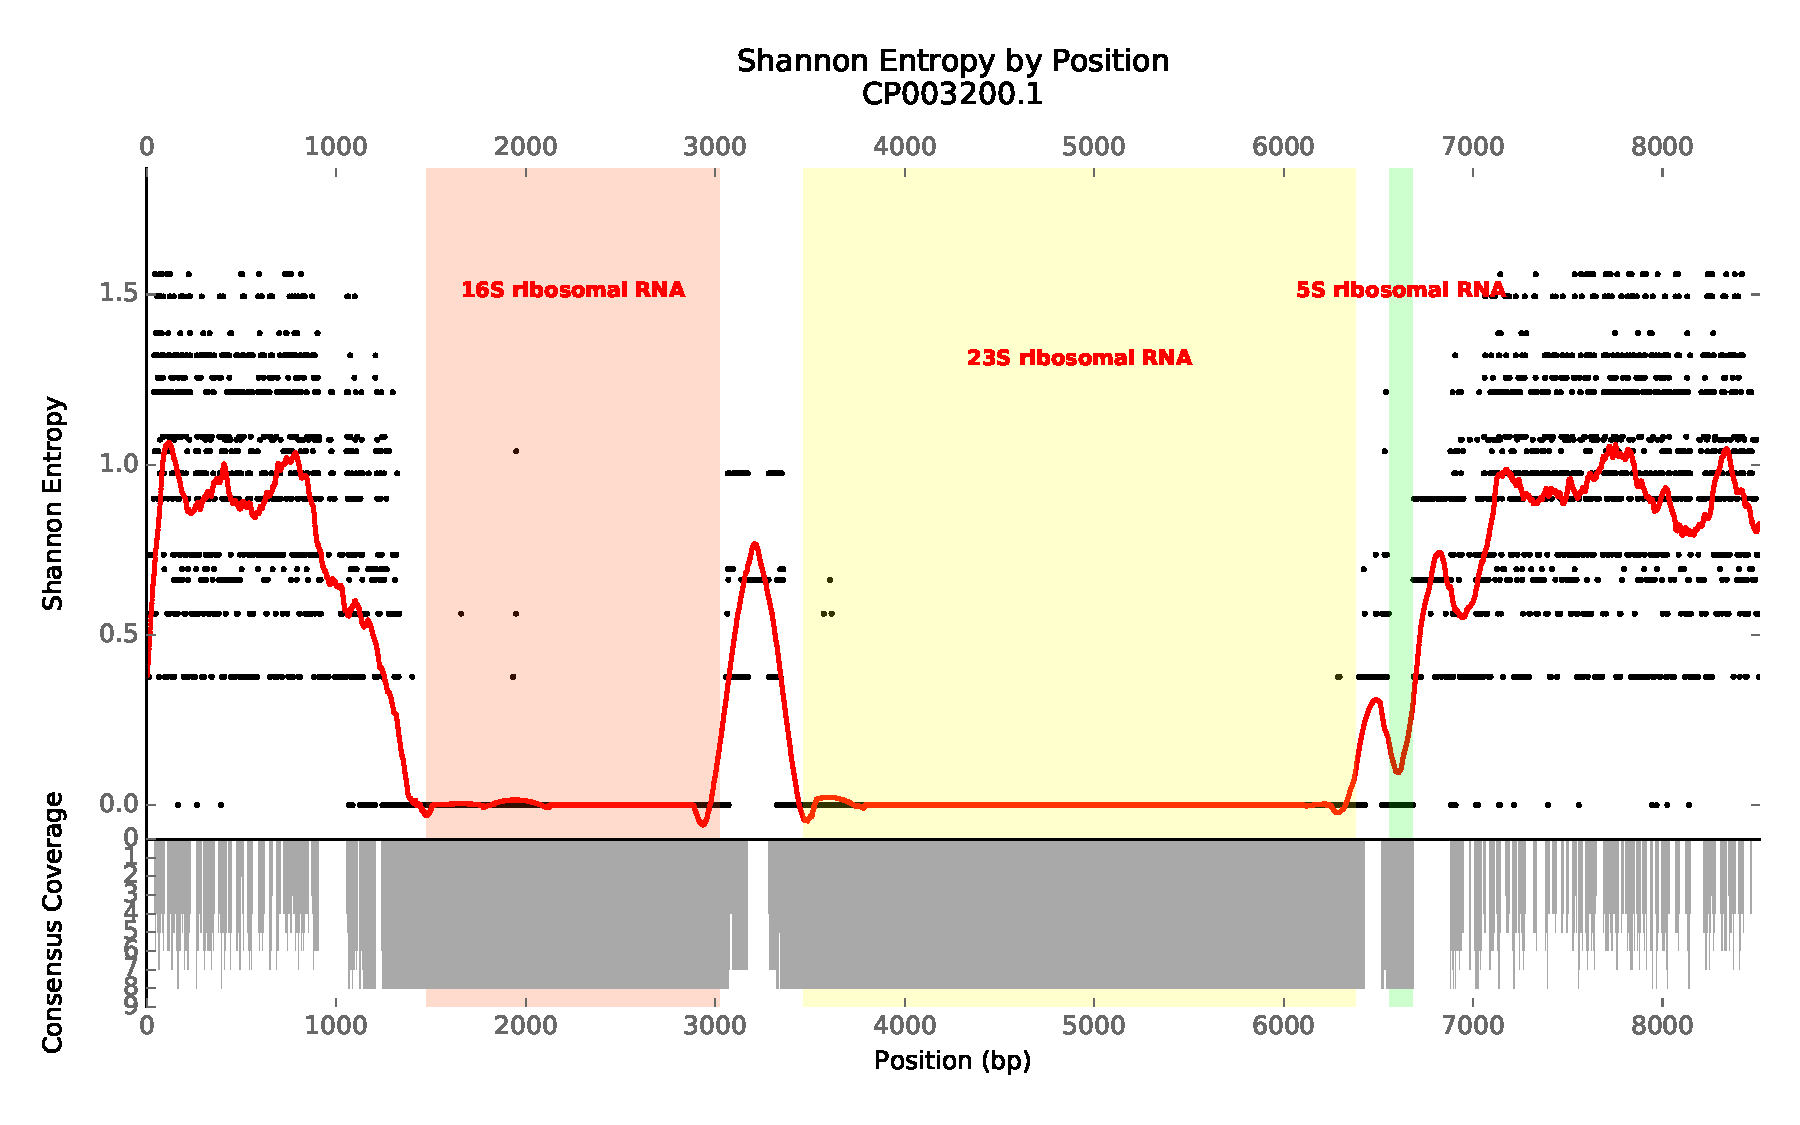
\includegraphics[width=0.95\textwidth]{gage_entropy_figures/CP003200.1_entropy_plot}
    \caption{\textit{K. pneumoniae subsp. pneumoniae HS11286} (CP003200.1) }
    \label{fig:ent_pneumo}
  \end{subfigure}
  \begin{subfigure}[b]{.45\textwidth}
    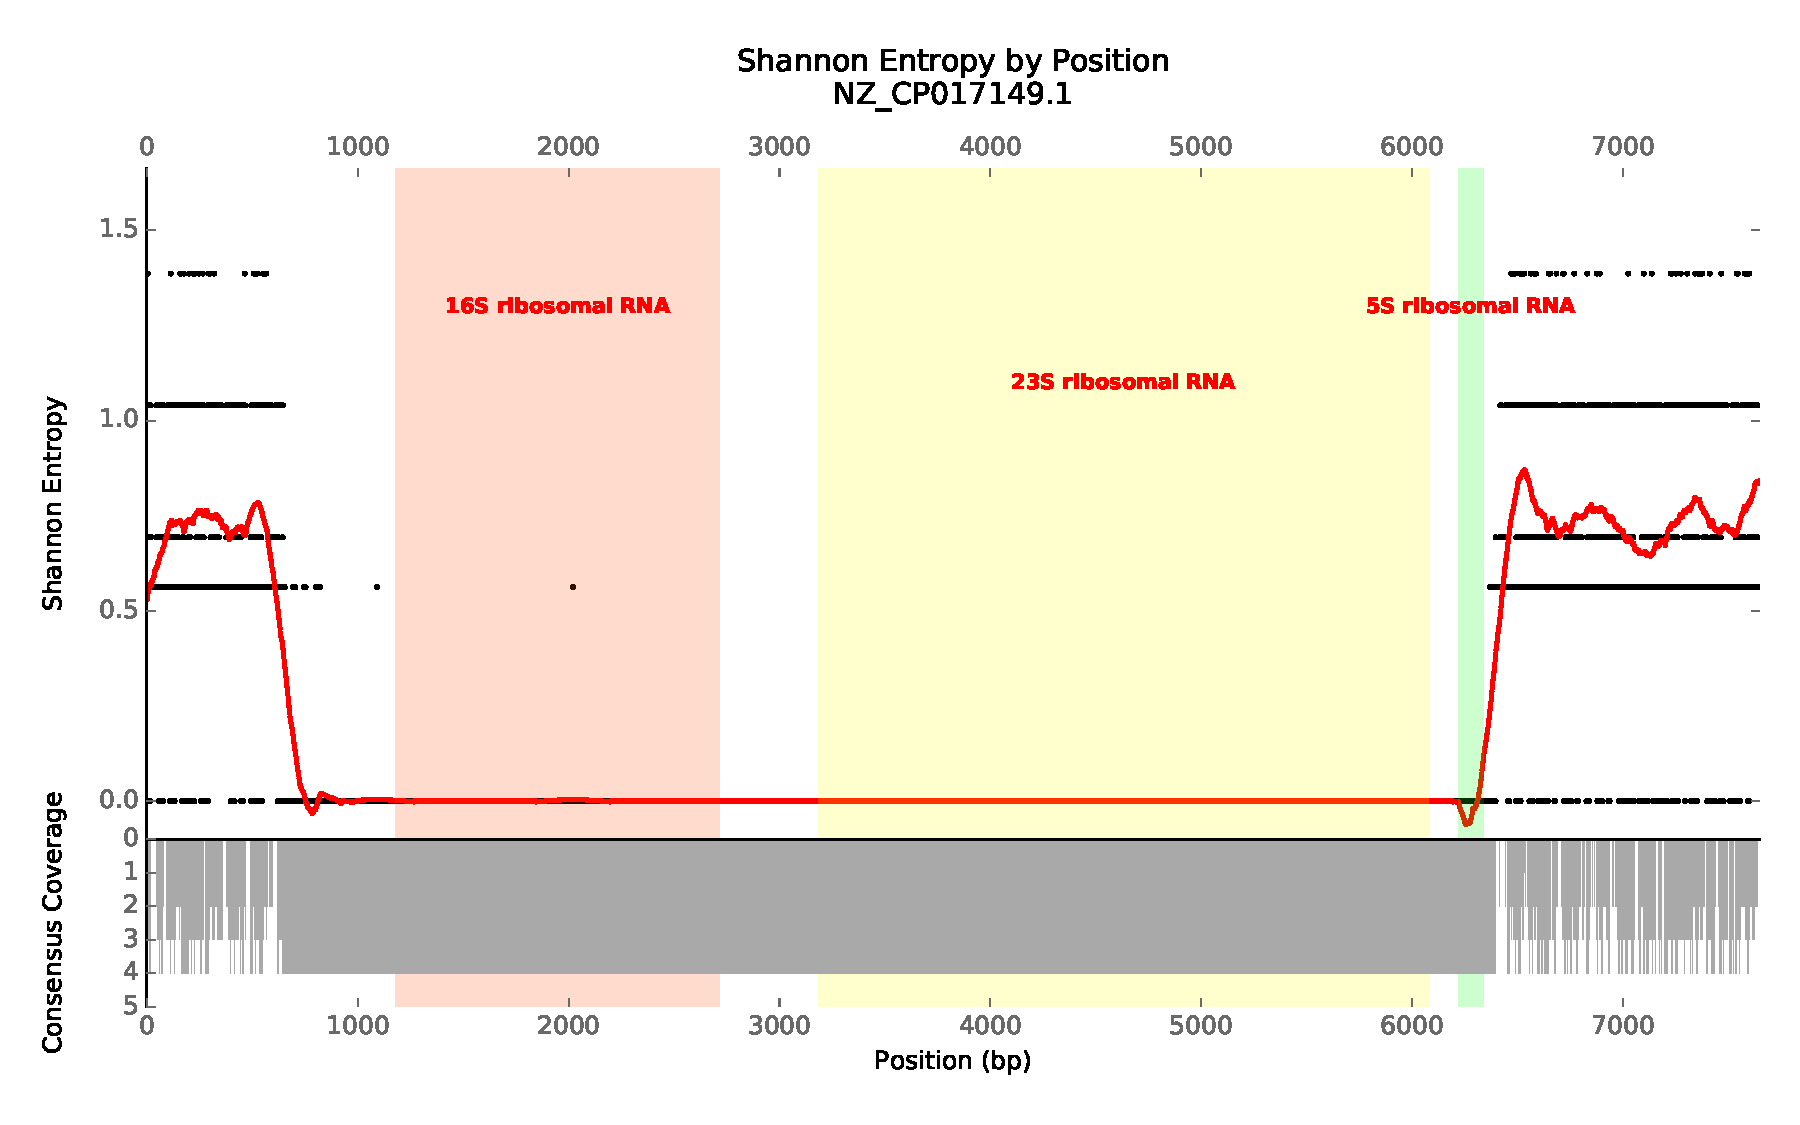
\includegraphics[width=0.95\textwidth]{gage_entropy_figures/NZ_CP017149.1_entropy_plot}
    \caption{\textit{P. aeruginosa strain ATCC 15692} (NZ\_CP017149.1)}
    \label{fig:ent_pao}
  \end{subfigure}
  \begin{subfigure}[b]{.45\textwidth}
    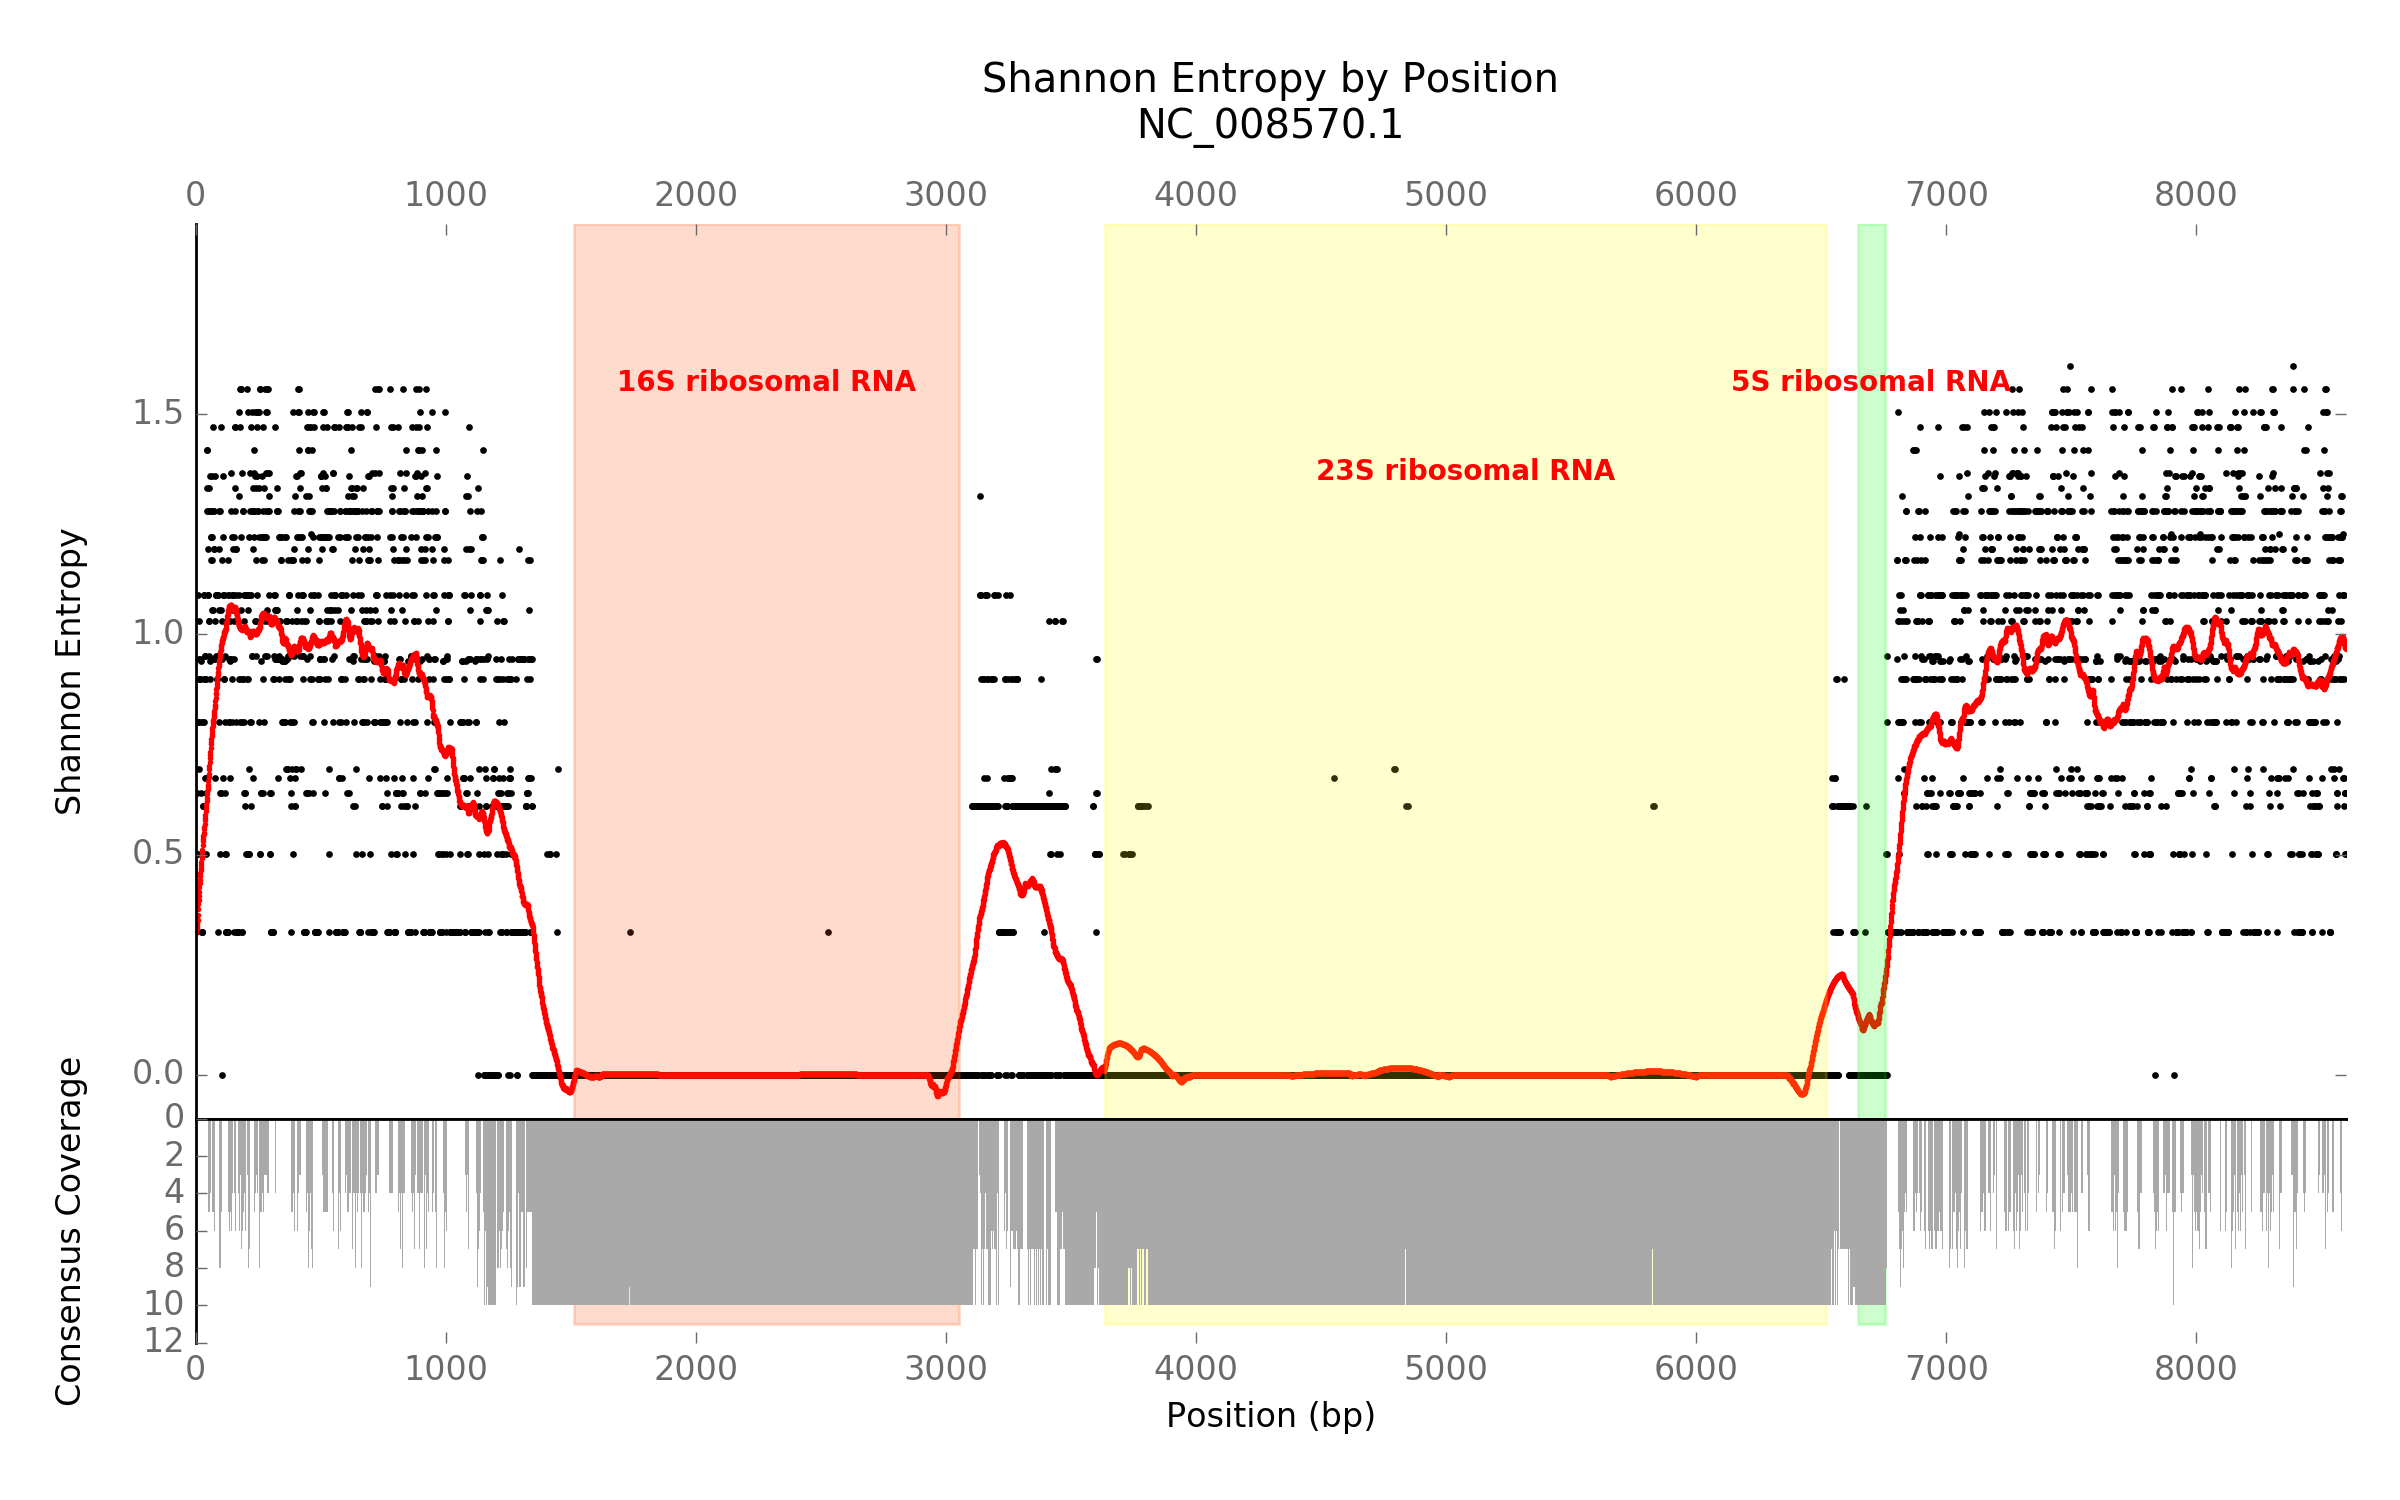
\includegraphics[width=0.95\textwidth]{gage_entropy_figures/NC_008570.1_entropy_plot}
    \caption{\textit{A. hydrophila ATCC 7966} (NC\_008570.1)}
    \label{fig:ent_aero}
  \end{subfigure}
  \begin{subfigure}[b]{.45\textwidth}
    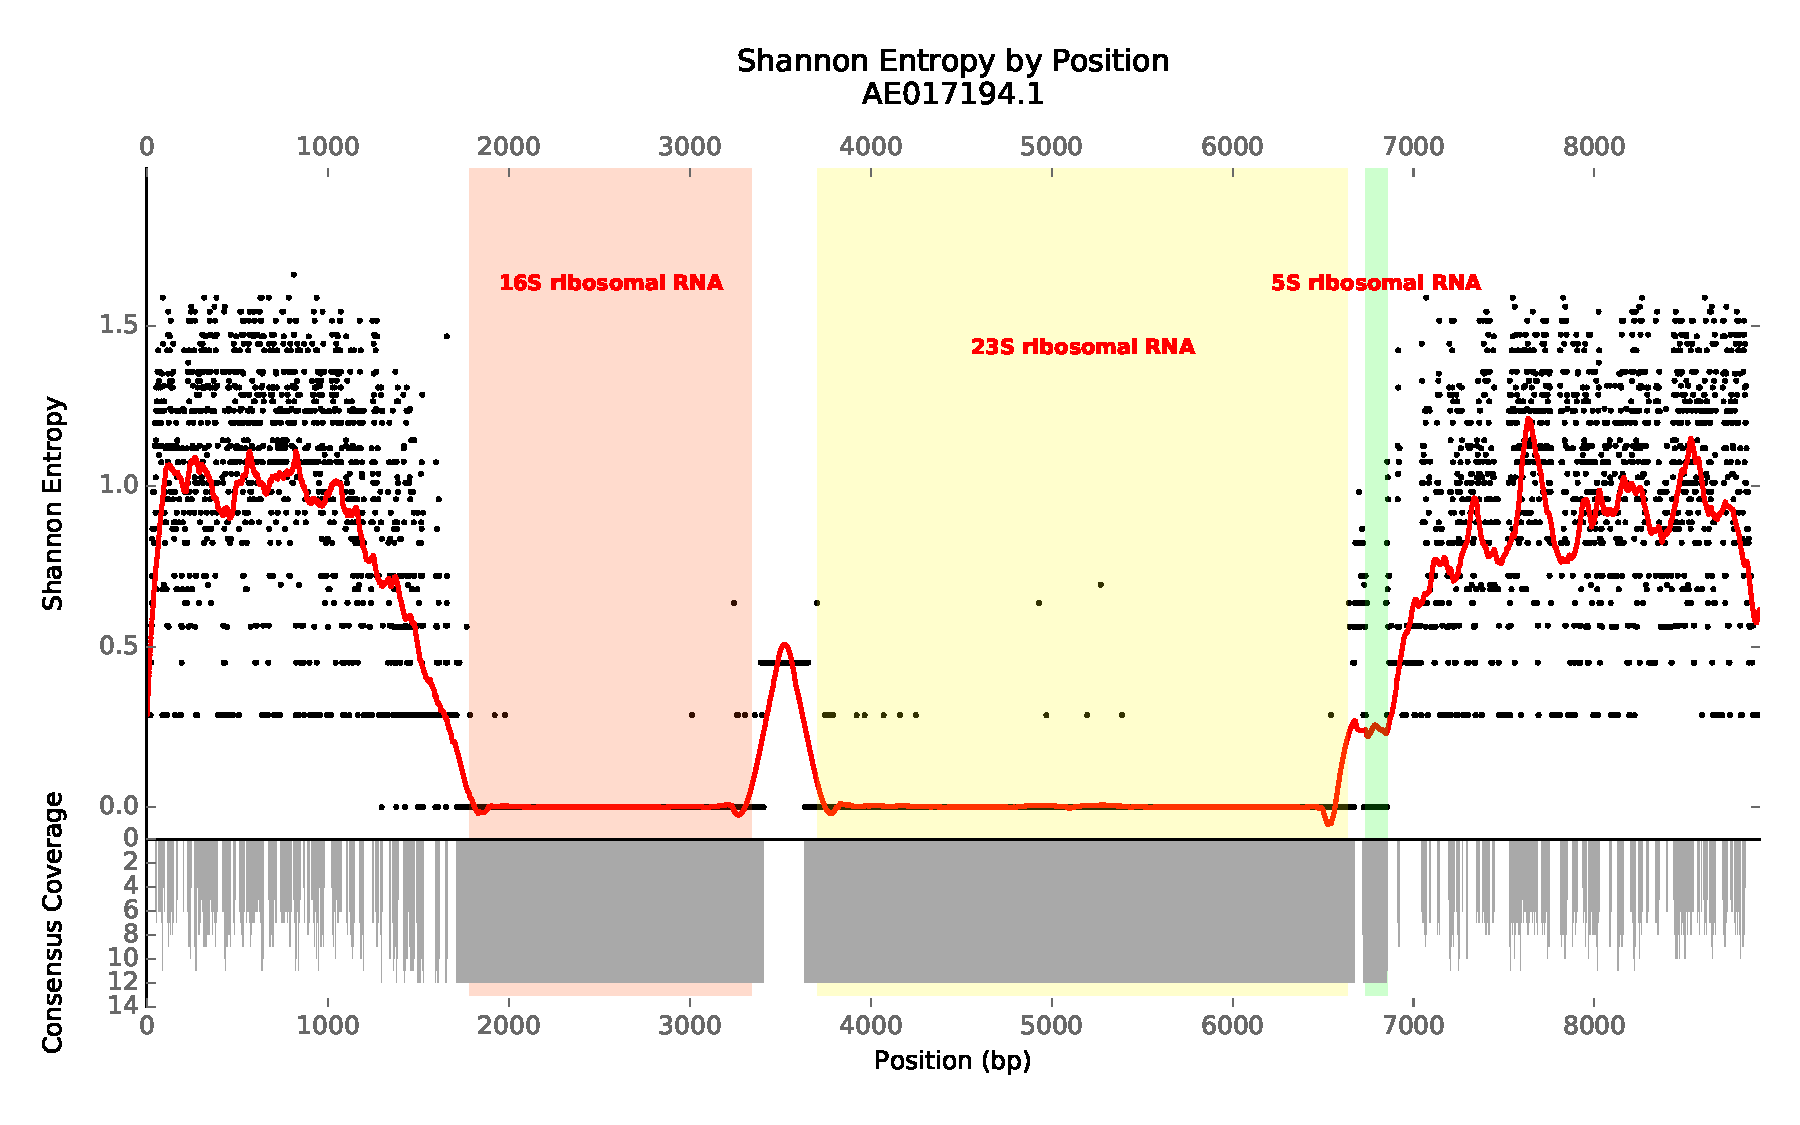
\includegraphics[width=0.95\textwidth]{gage_entropy_figures/AE017194.1_entropy_plot}
    \caption{\textit{B. cereus ATCC 10987} (AE017194.1)}
    \label{fig:ent_cereus_atcc}
  \end{subfigure}
  \begin{subfigure}[b]{.45\textwidth}
    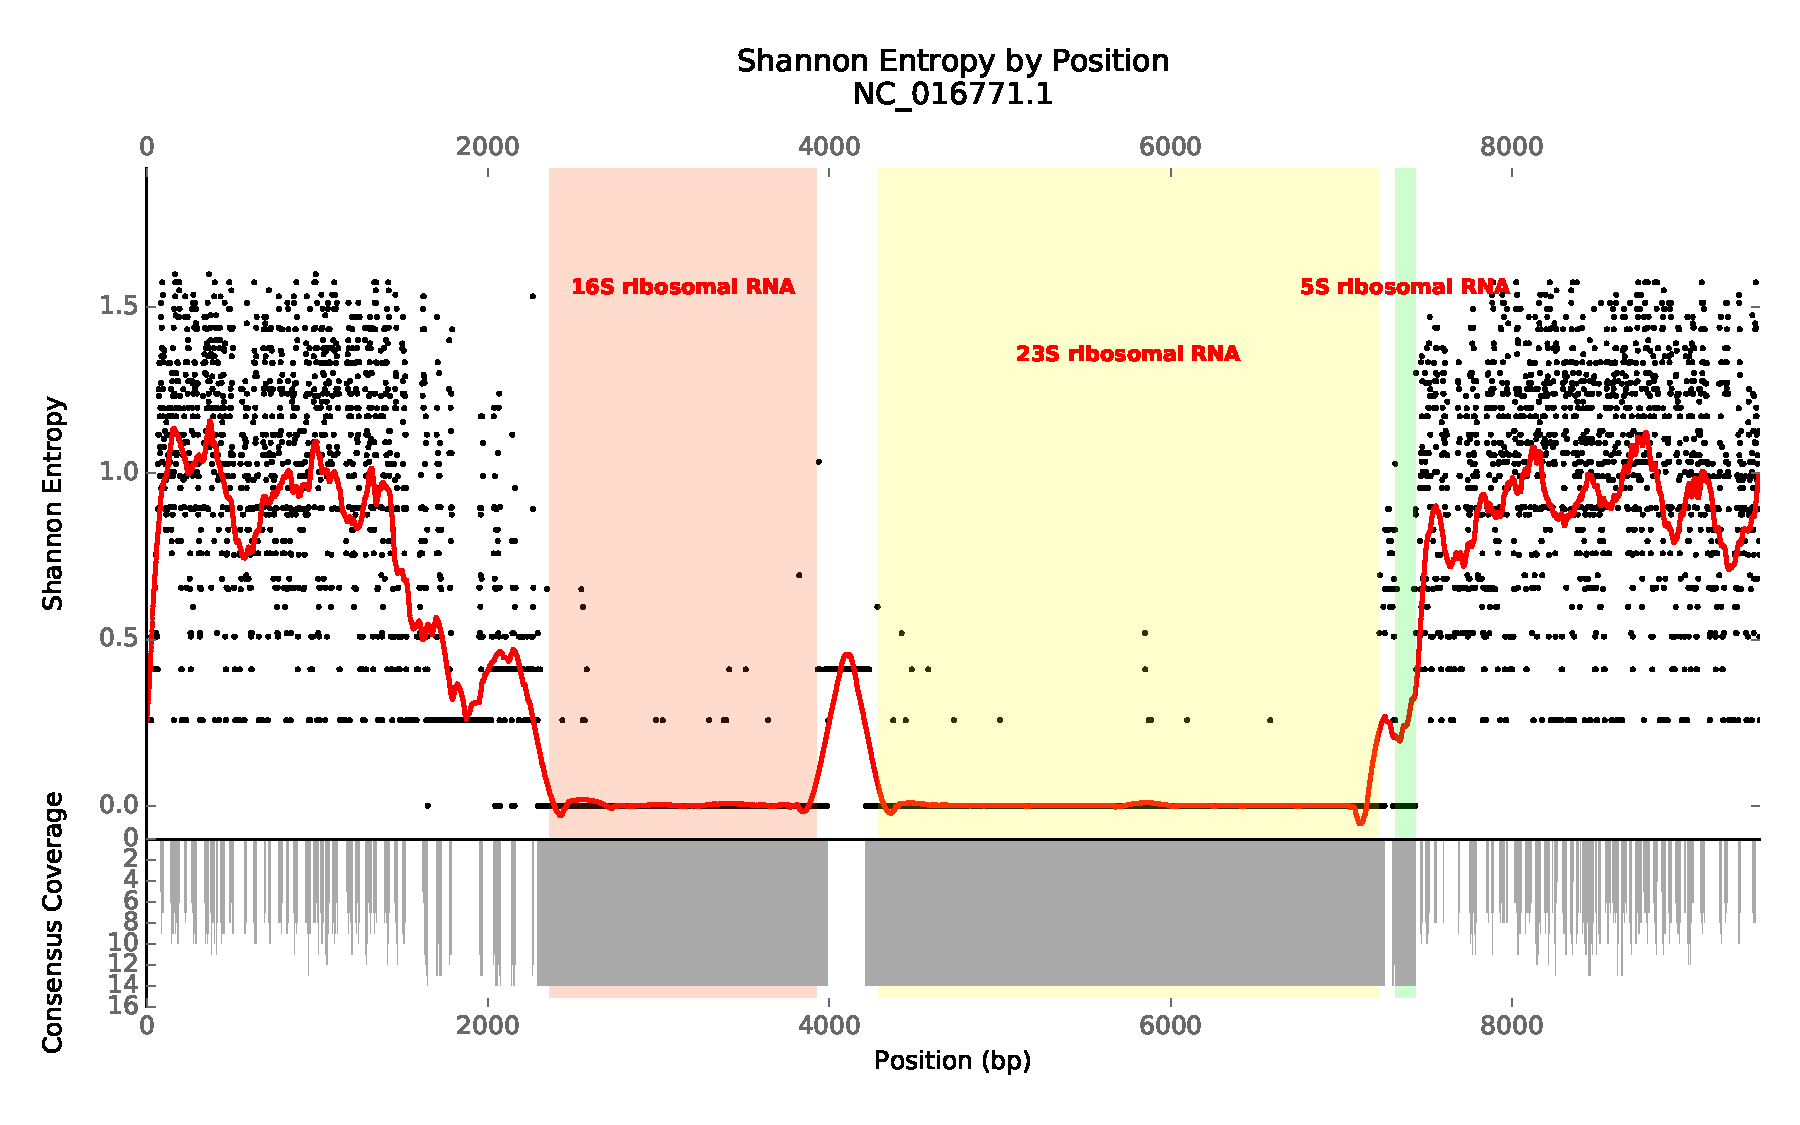
\includegraphics[width=0.95\textwidth]{gage_entropy_figures/NC_016771.1_entropy_plot}
    \caption{\textit{B. cereus NC7401} (NC\_016771.1)}
    \label{fig:ent_cereus_nc}
  \end{subfigure}
  \begin{subfigure}[b]{.45\textwidth}
    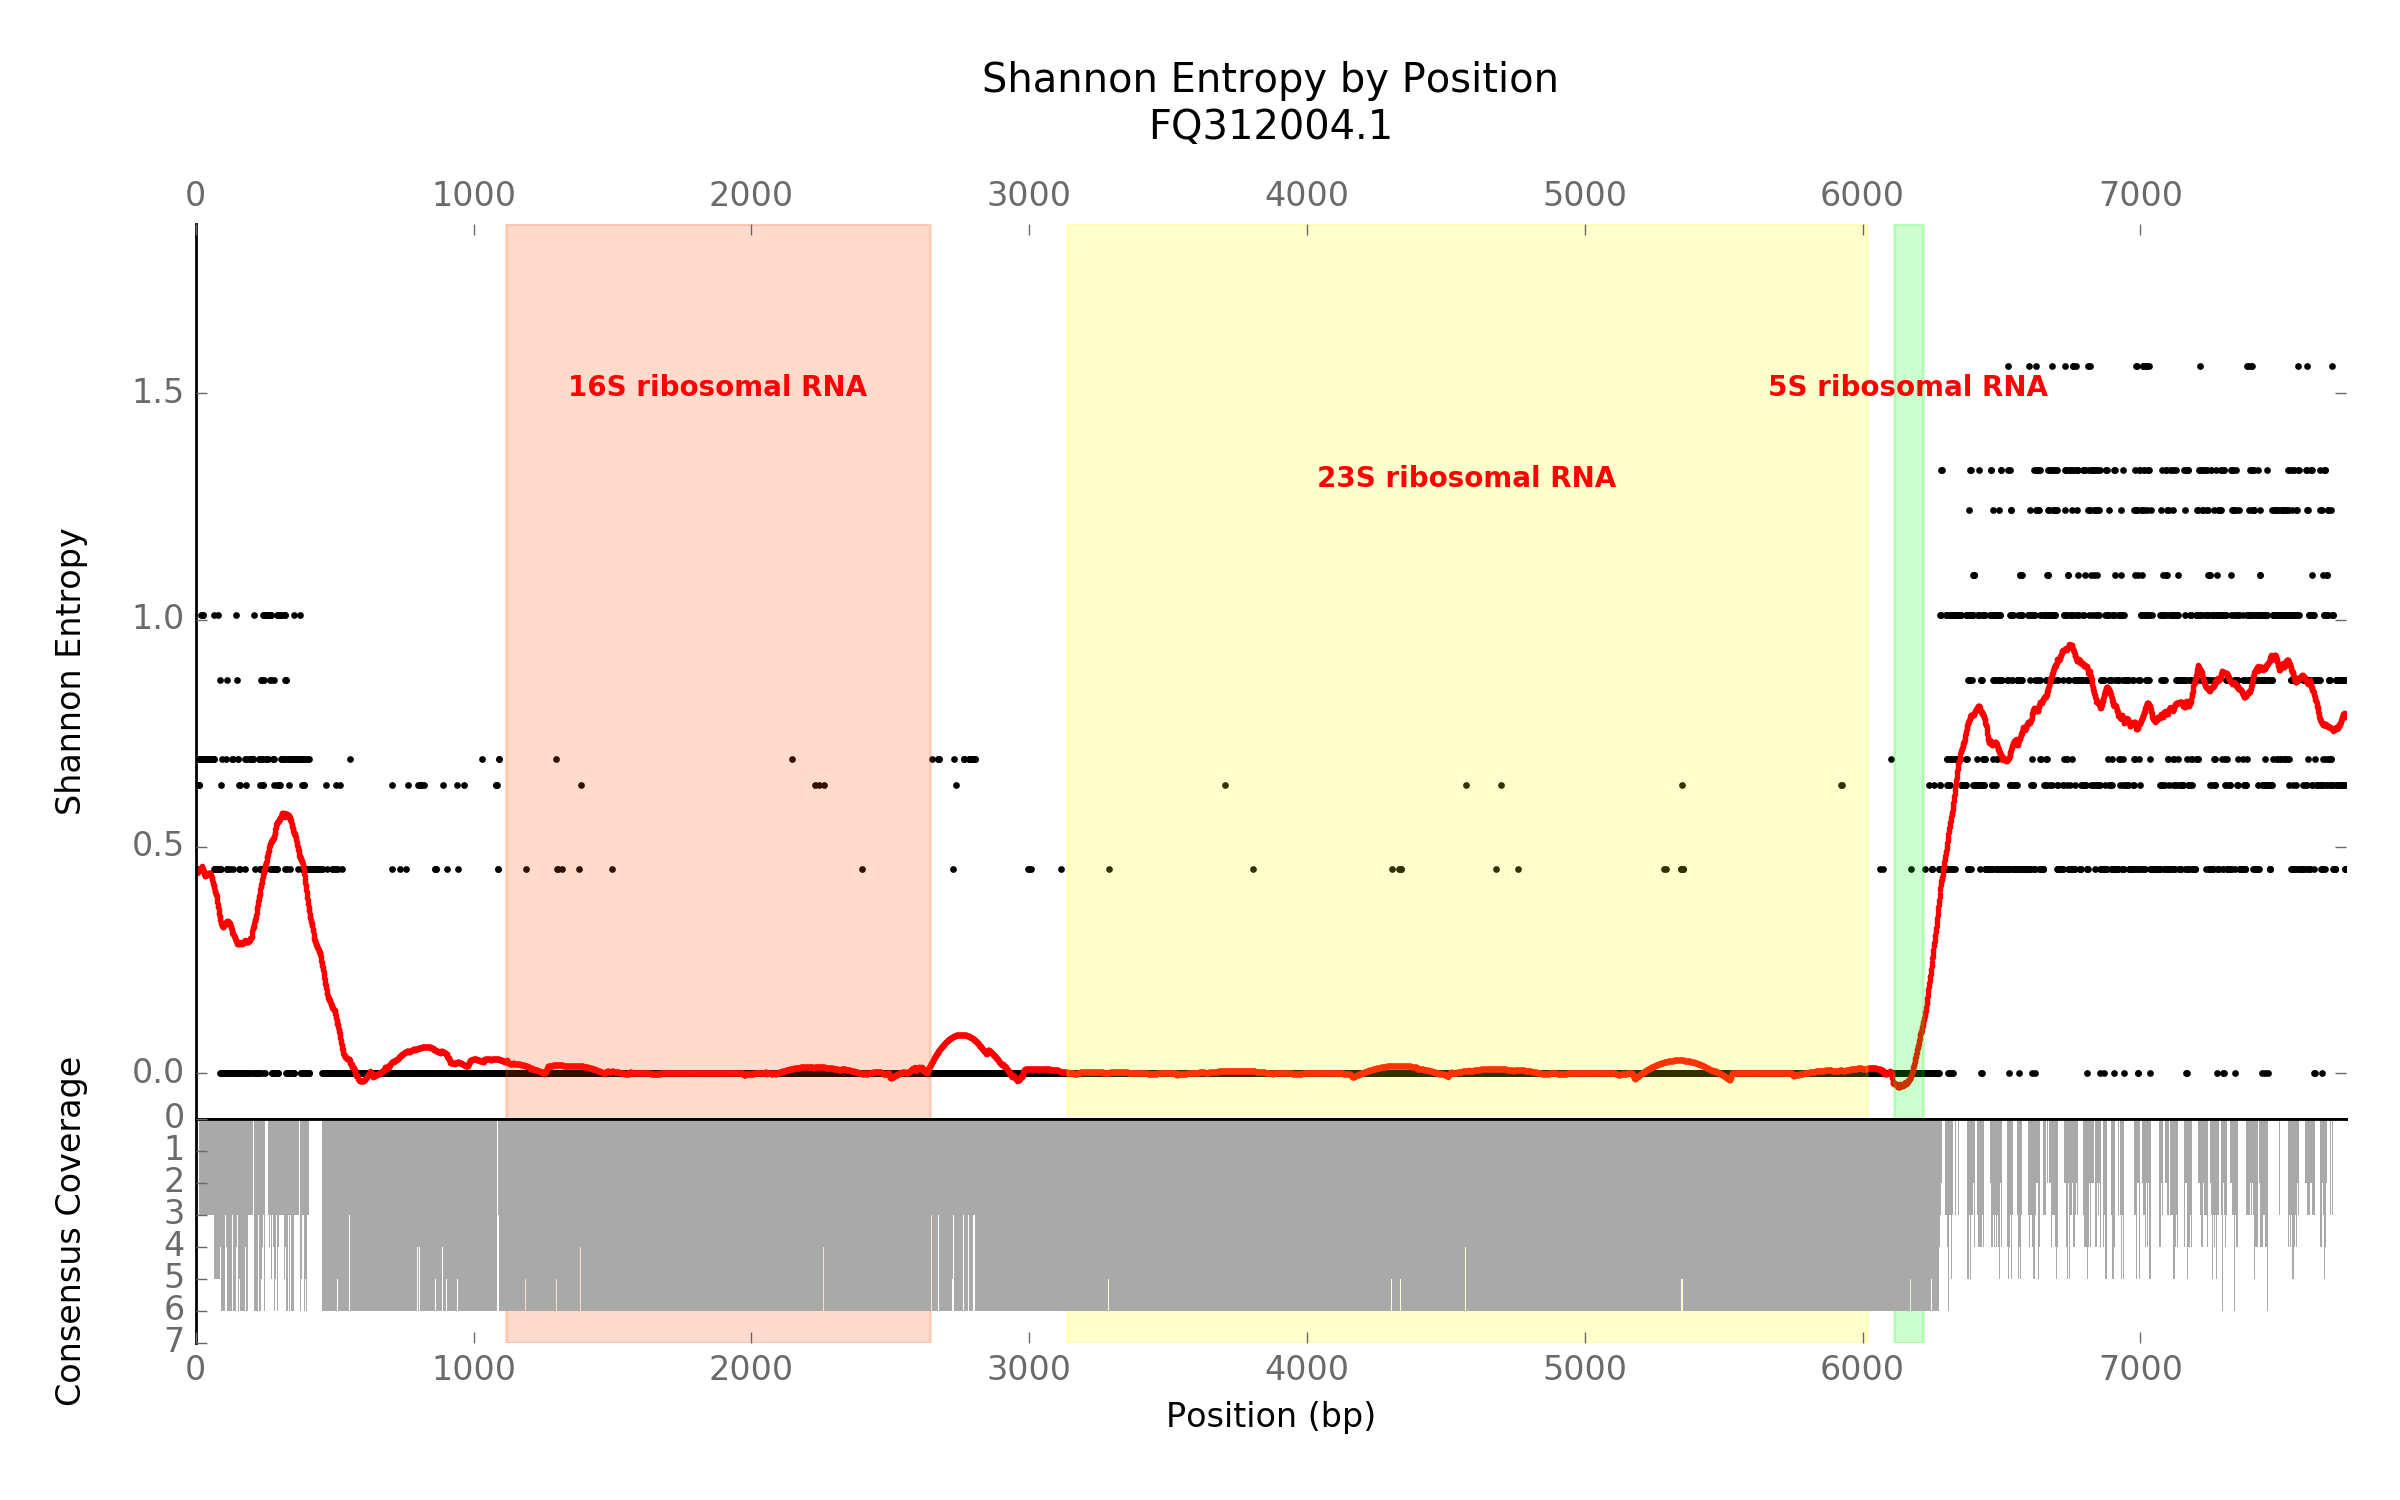
\includegraphics[width=0.95\textwidth]{gage_entropy_figures/FQ312004.1_entropy_plot}
    \caption{\textit{B. fragilis 638R} (FQ312004.1)}
    \label{fig:ent_frag}
  \end{subfigure}
  \begin{subfigure}[b]{.45\textwidth}
    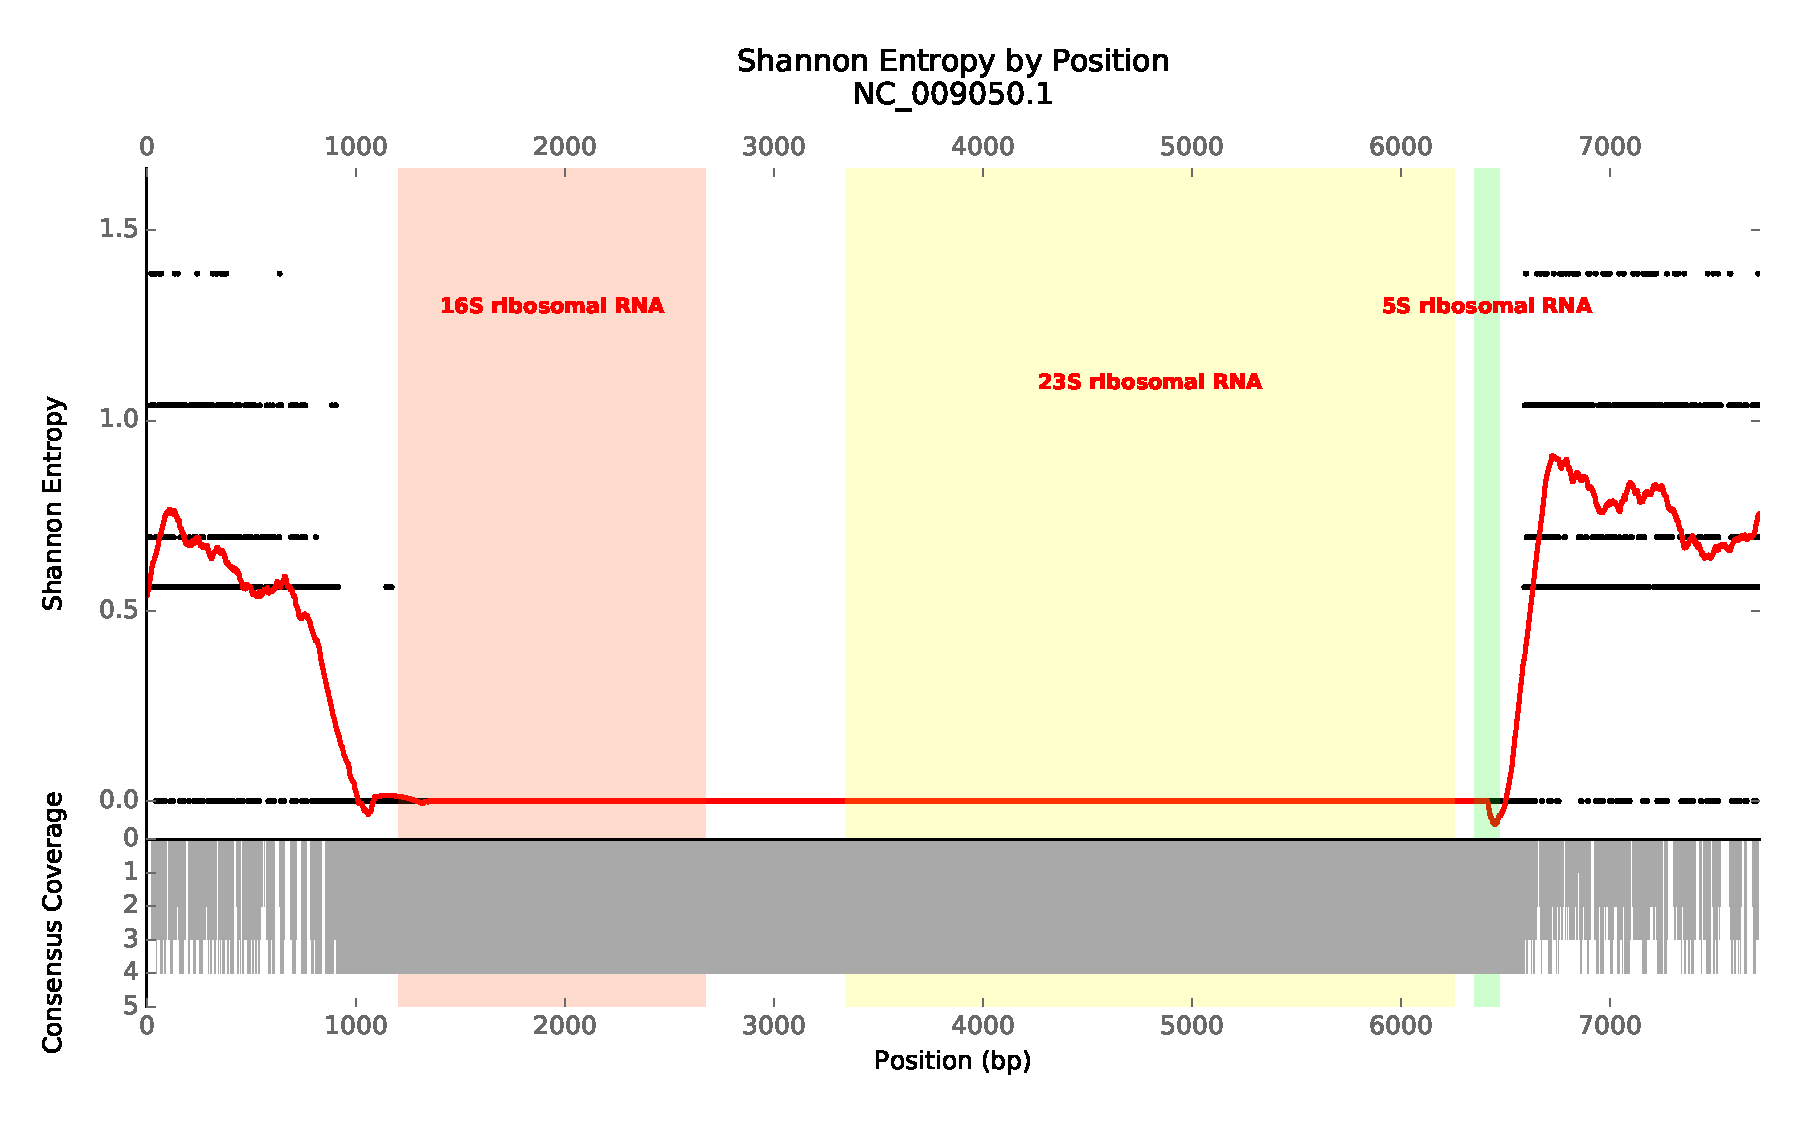
\includegraphics[width=0.95\textwidth]{gage_entropy_figures/NC_009050.1_entropy_plot}
    \caption{\textit{R. sphaeroides  ATCC 17029} (NC\_009049.1, NC\_009050.1)}
    \label{fig:ent_rhodo}
  \end{subfigure}
\end{figure}
\begin{figure}
  \centering
  \ContinuedFloat
  \begin{subfigure}[b]{.45\textwidth}
    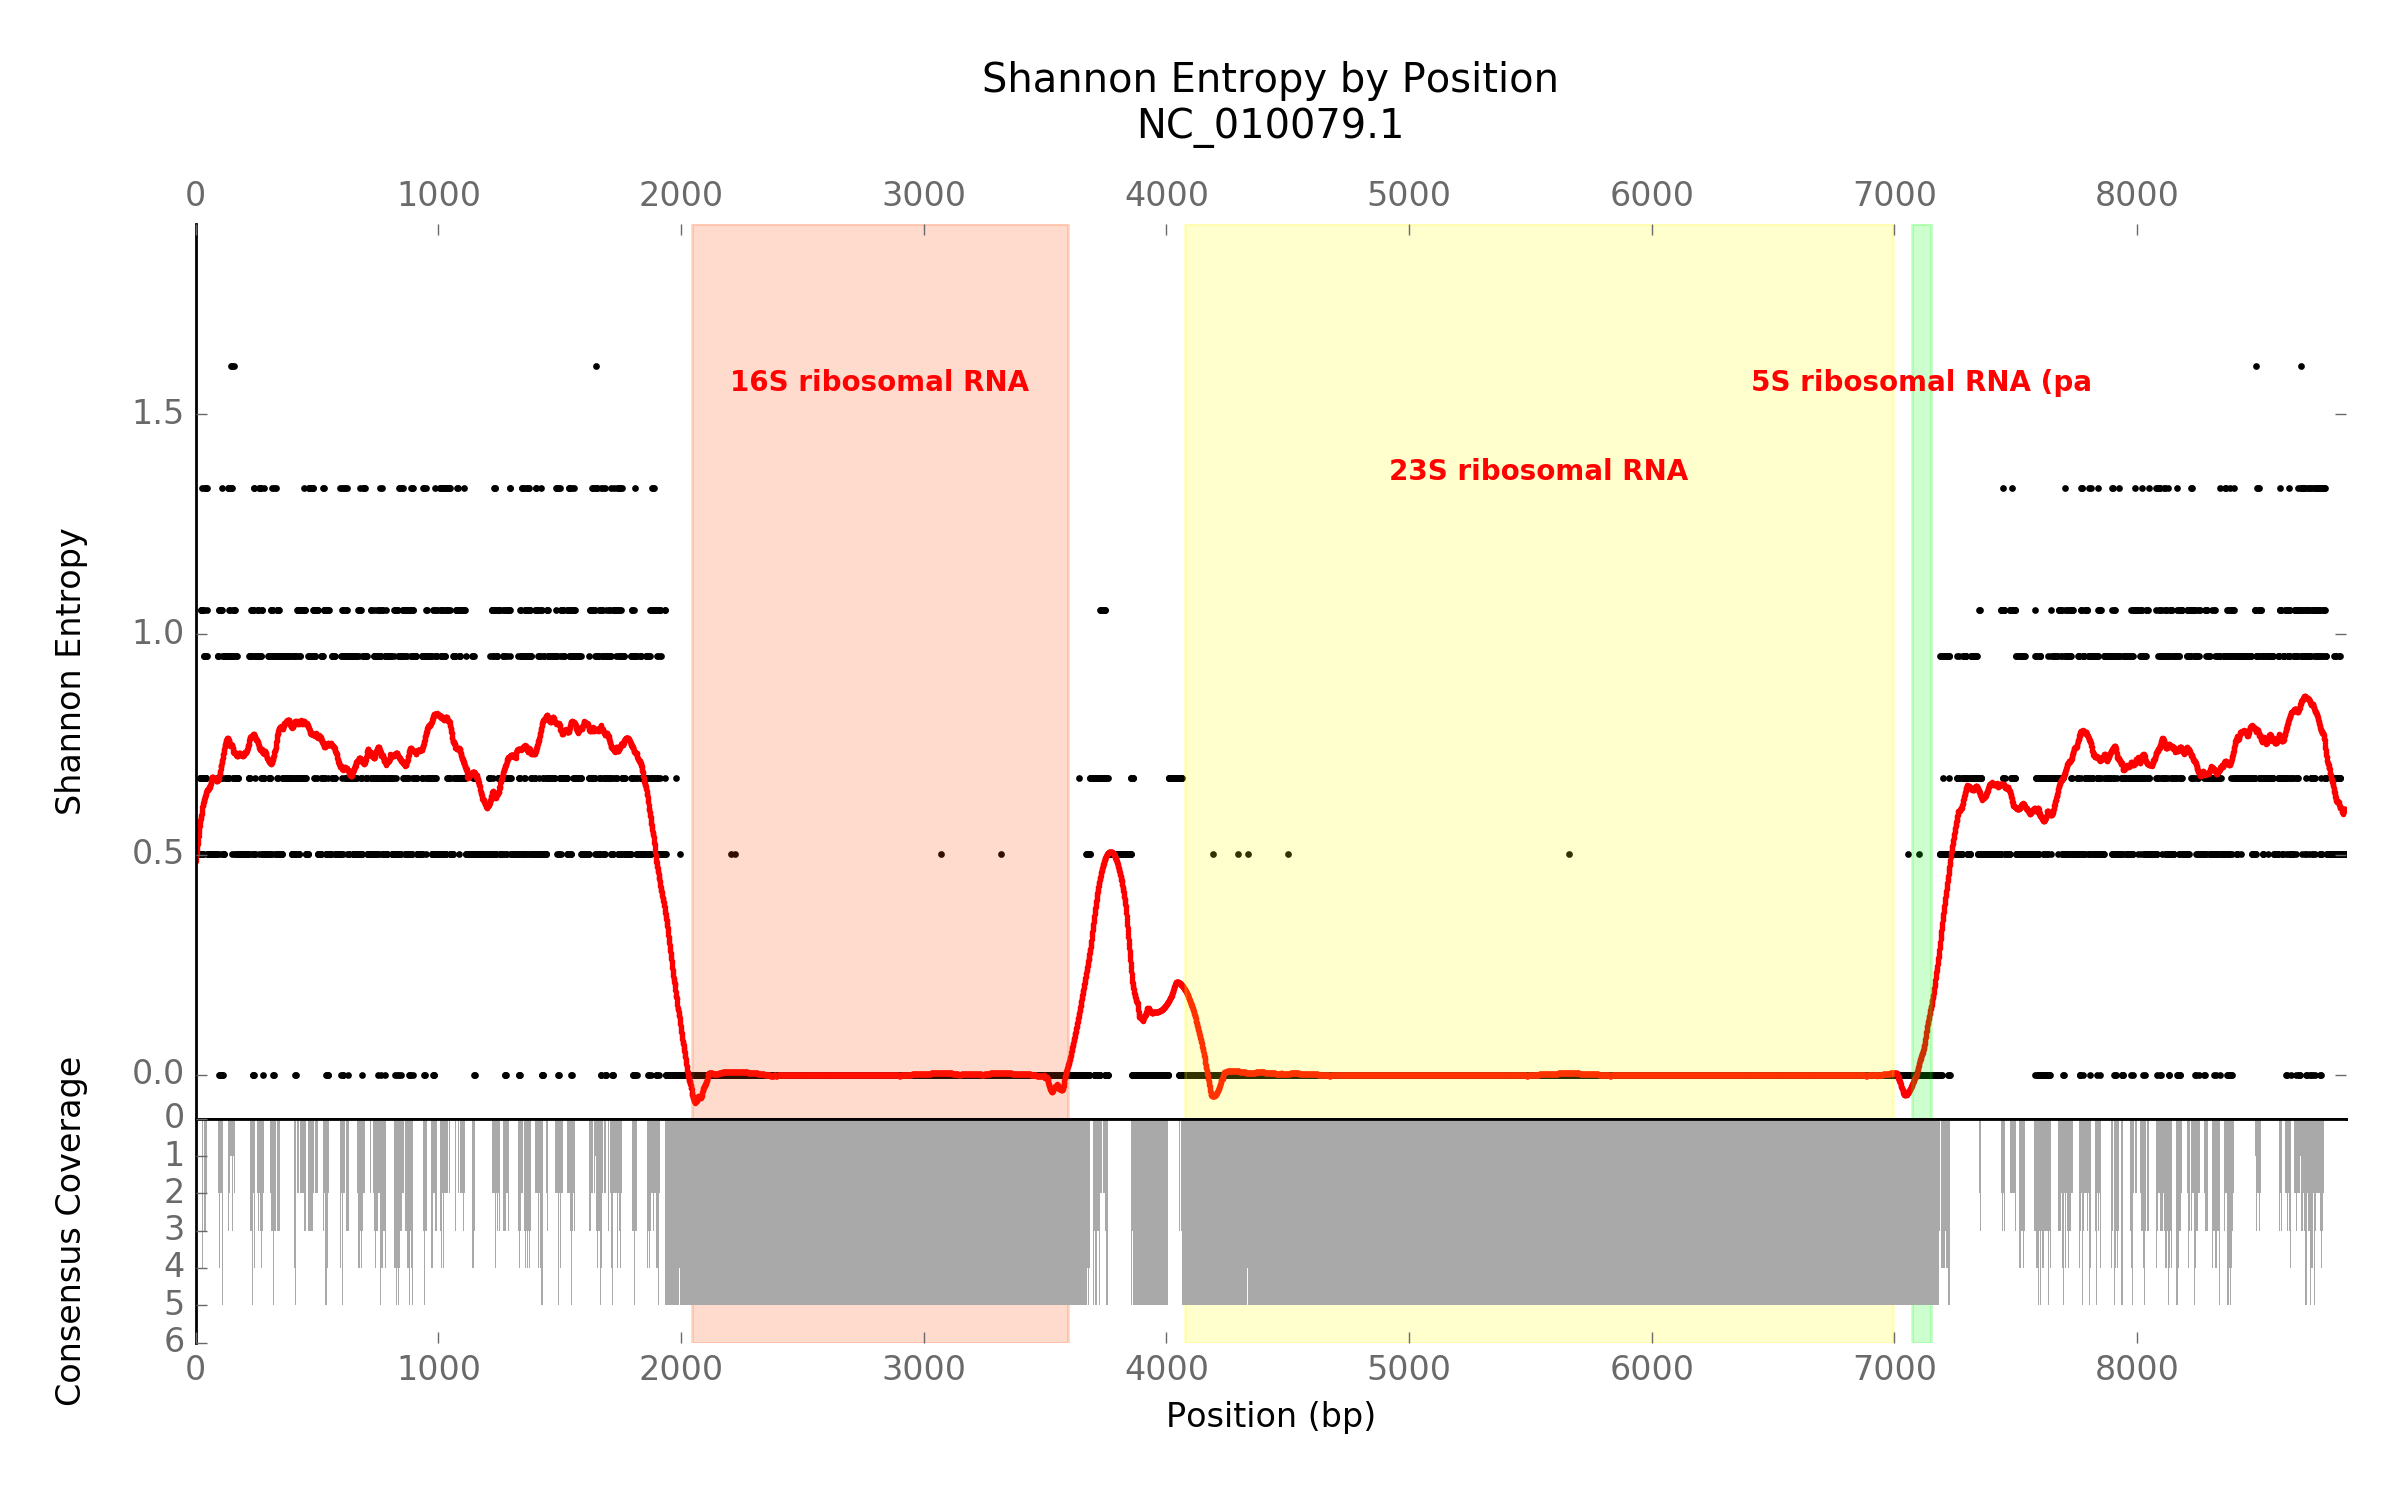
\includegraphics[width=0.95\textwidth]{gage_entropy_figures/NC_010079.1_entropy_plot}
    \caption{\textit{S. aureus TCH1516} (NC\_010079.1)}
    \label{fig:ent_tch}
  \end{subfigure}
  % \begin{subfigure}[b]{.45\textwidth}
  %   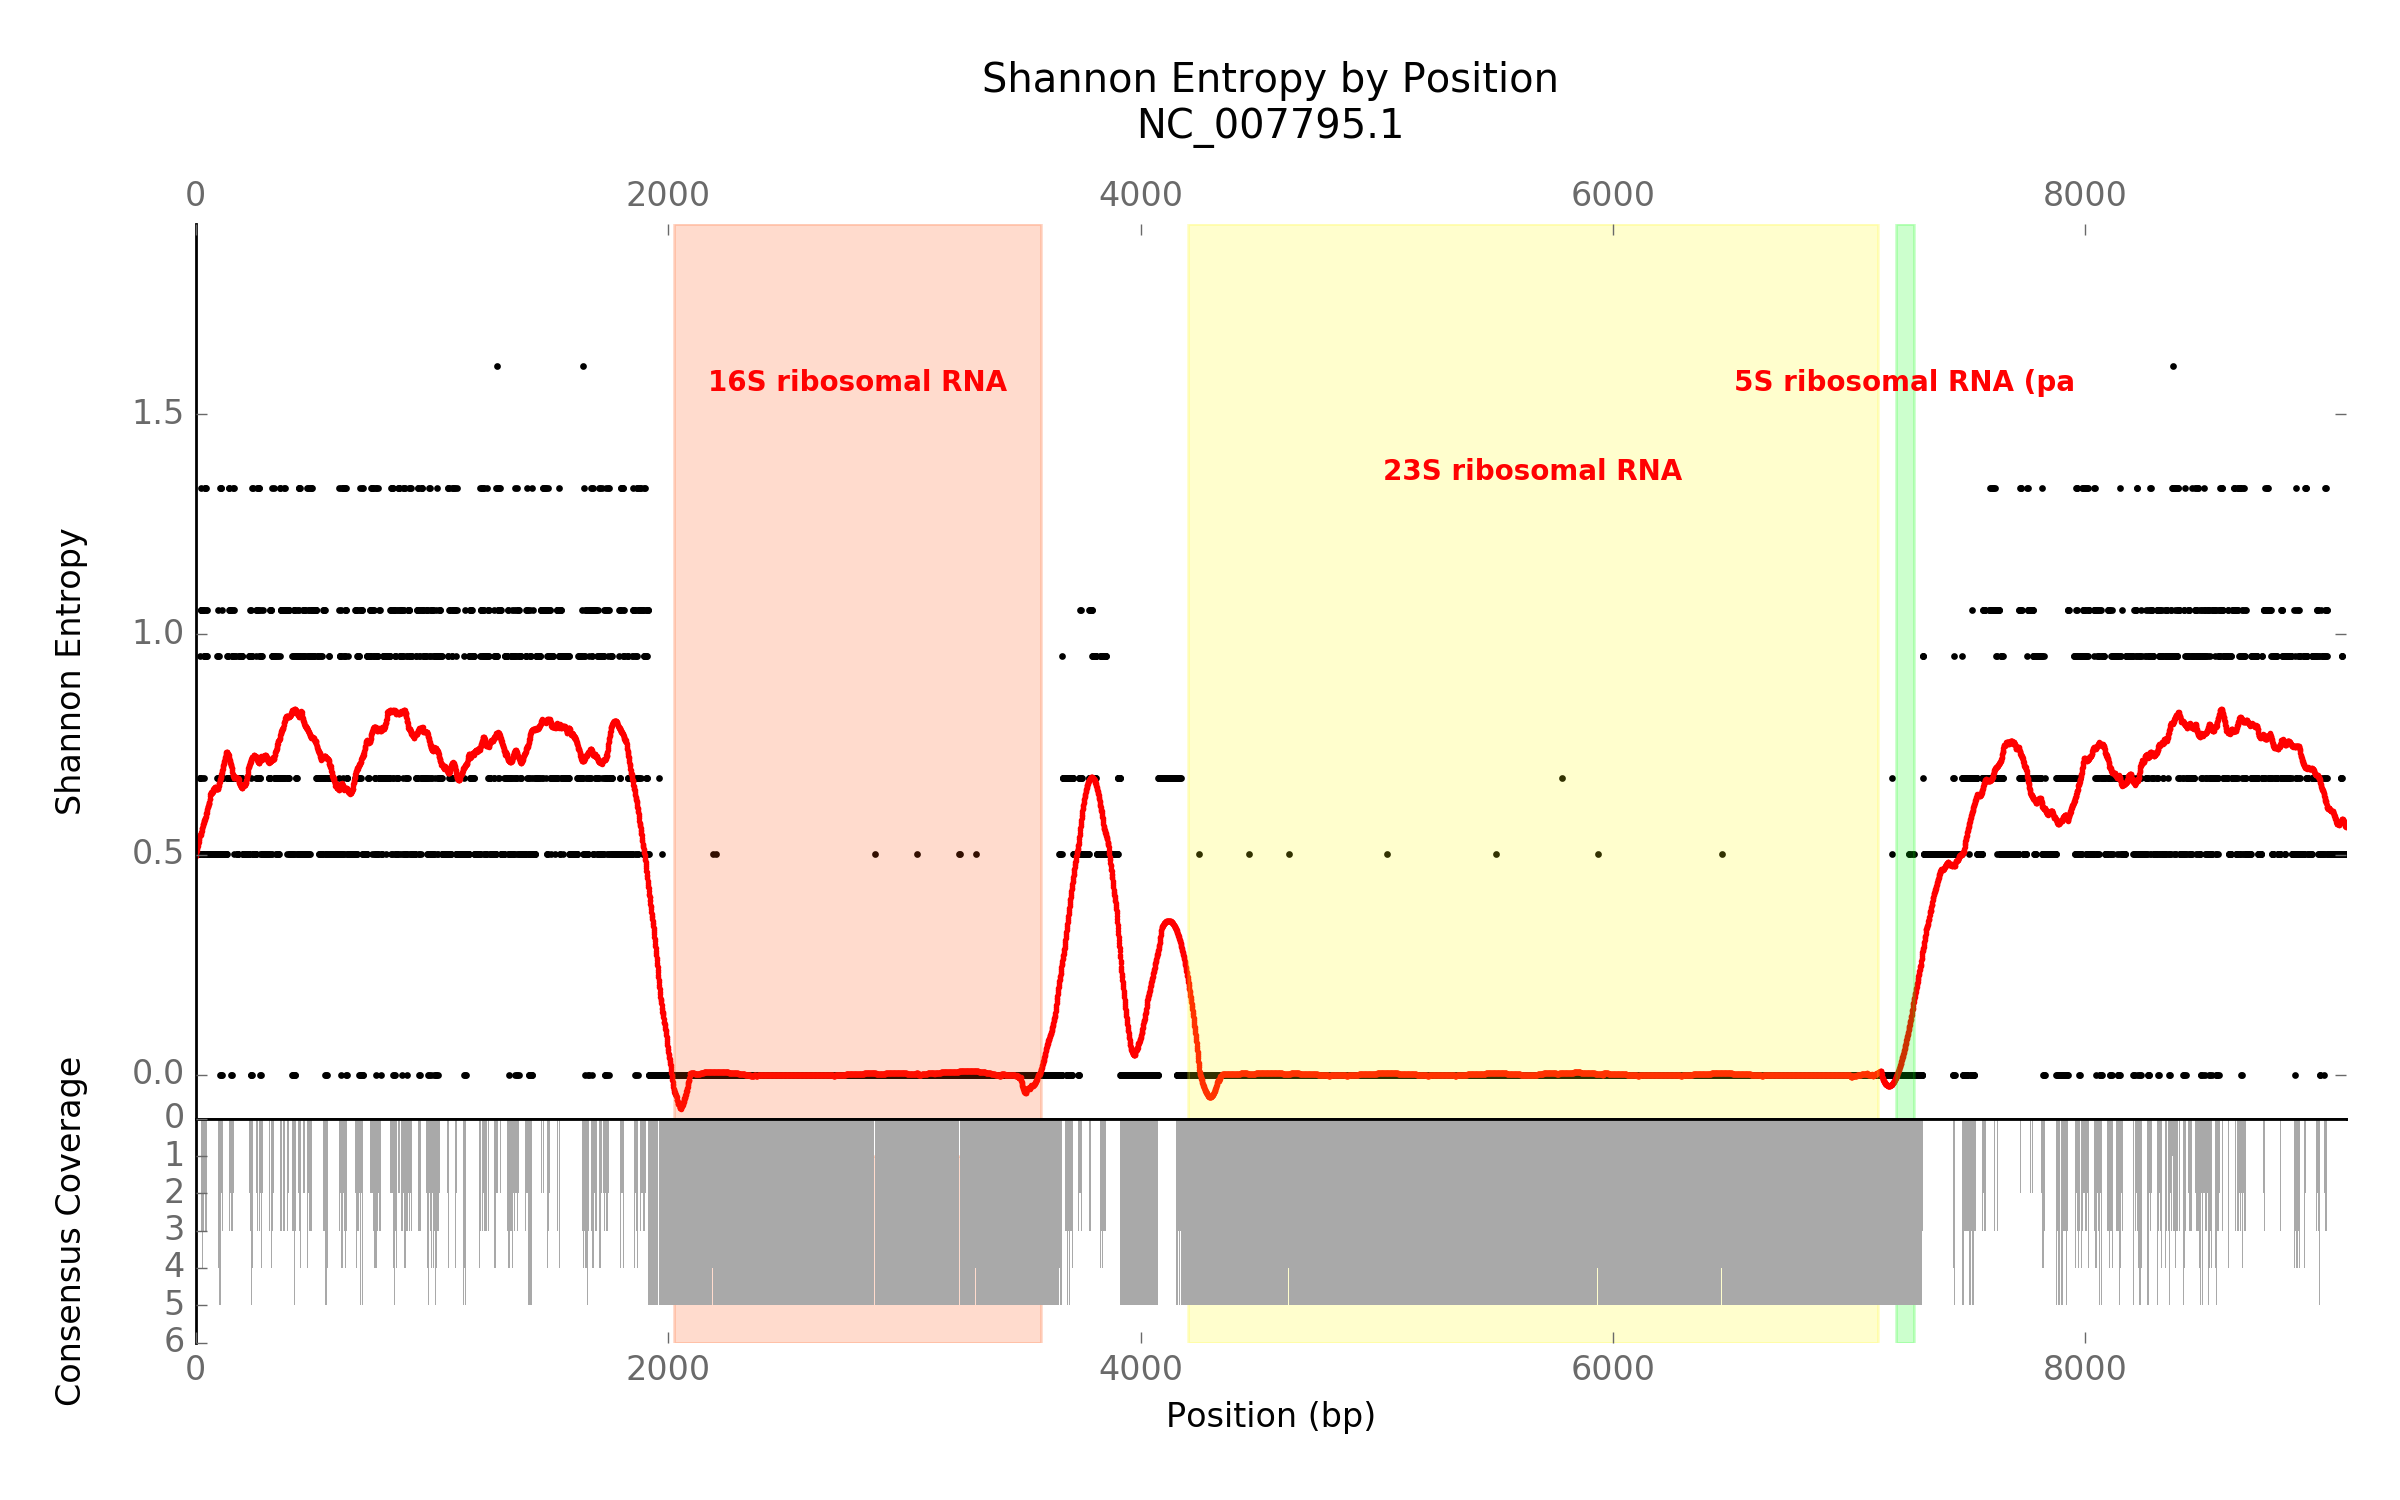
\includegraphics[width=0.95\textwidth]{gage_entropy_figures/NC_007795.1_entropy_plot}
  %   \caption{\textit{S. aureus NCTC 8325} (NC\_007795.1)}
  %   \label{fig:ent_nctc}
  % \end{subfigure}
  % \begin{subfigure}[b]{.45\textwidth}
  %   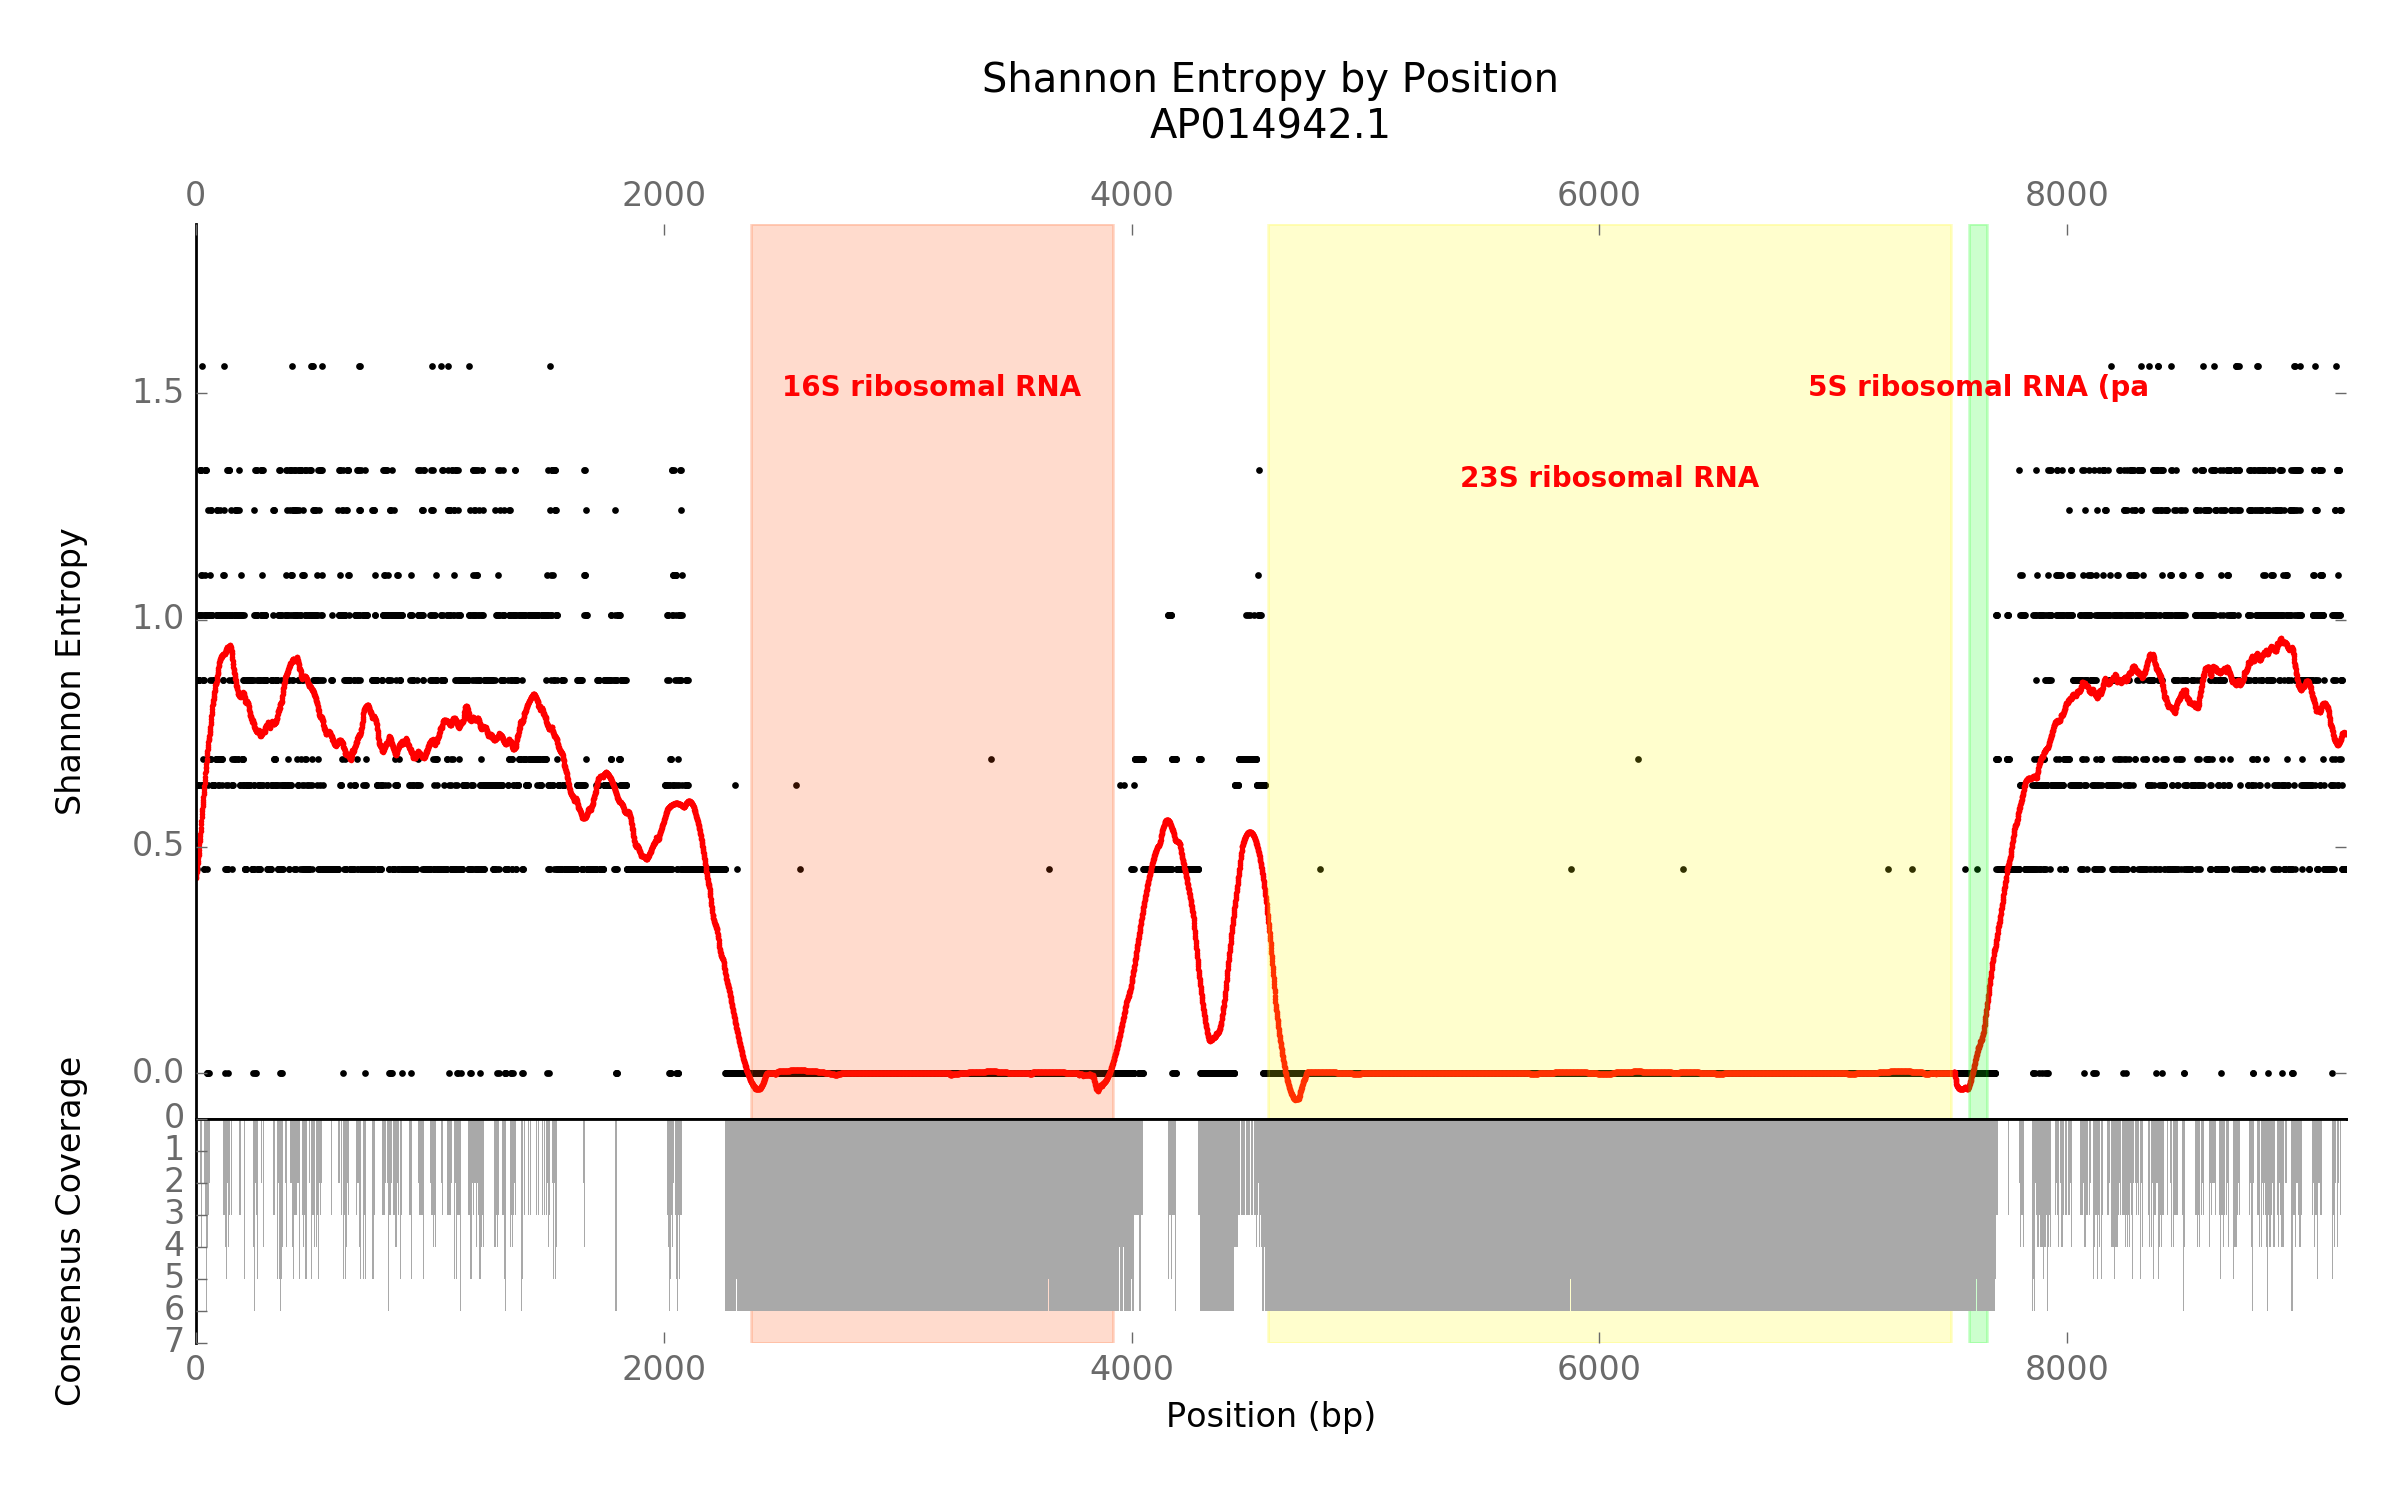
\includegraphics[width=0.95\textwidth]{gage_entropy_figures/AP014942.1_entropy_plot}
  % \caption{\textit{S. aureus FDA209P} (AP014942.1)}
  % \label{fig:entfda}
  % \end{subfigure}
  \begin{subfigure}[b]{.45\textwidth}
    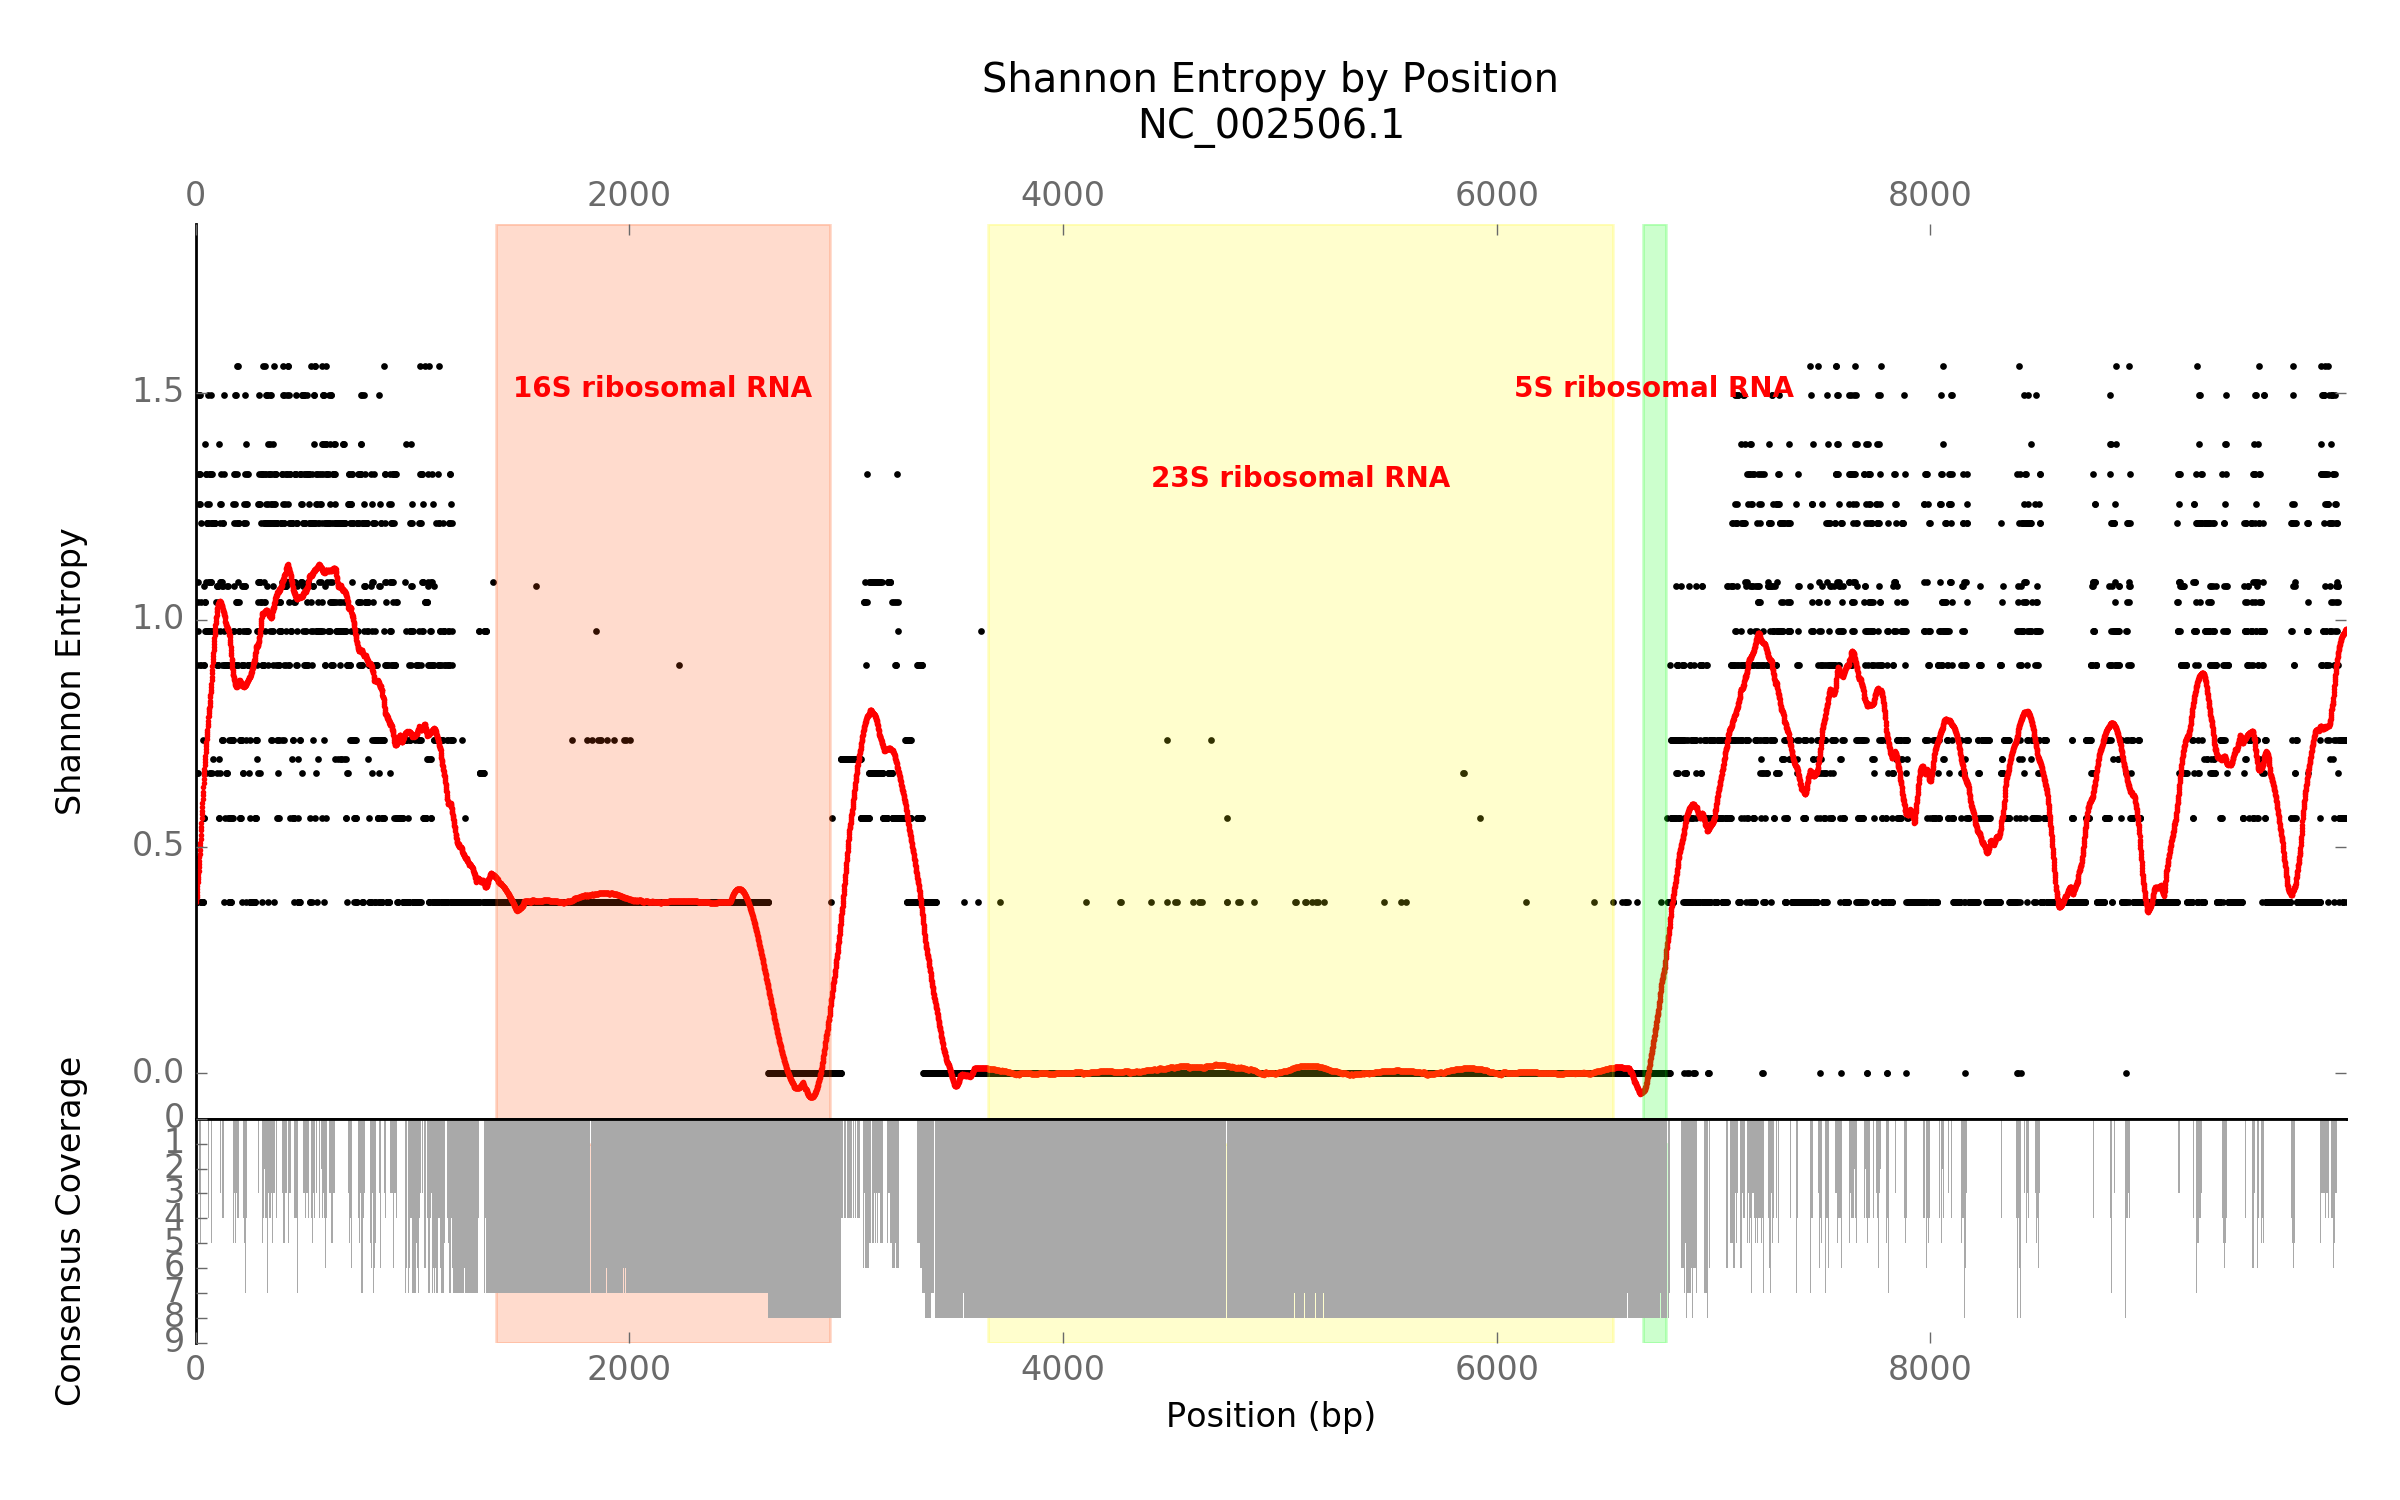
\includegraphics[width=0.95\textwidth]{gage_entropy_figures/NC_002506.1_entropy_plot}
    \caption{\textit{V. cholerae El Tor str. N16961} (NC\_002505.1) (NC\_002506.1)}
    \label{fig:ent_vib}
  \end{subfigure}
  \begin{subfigure}[b]{.45\textwidth}
    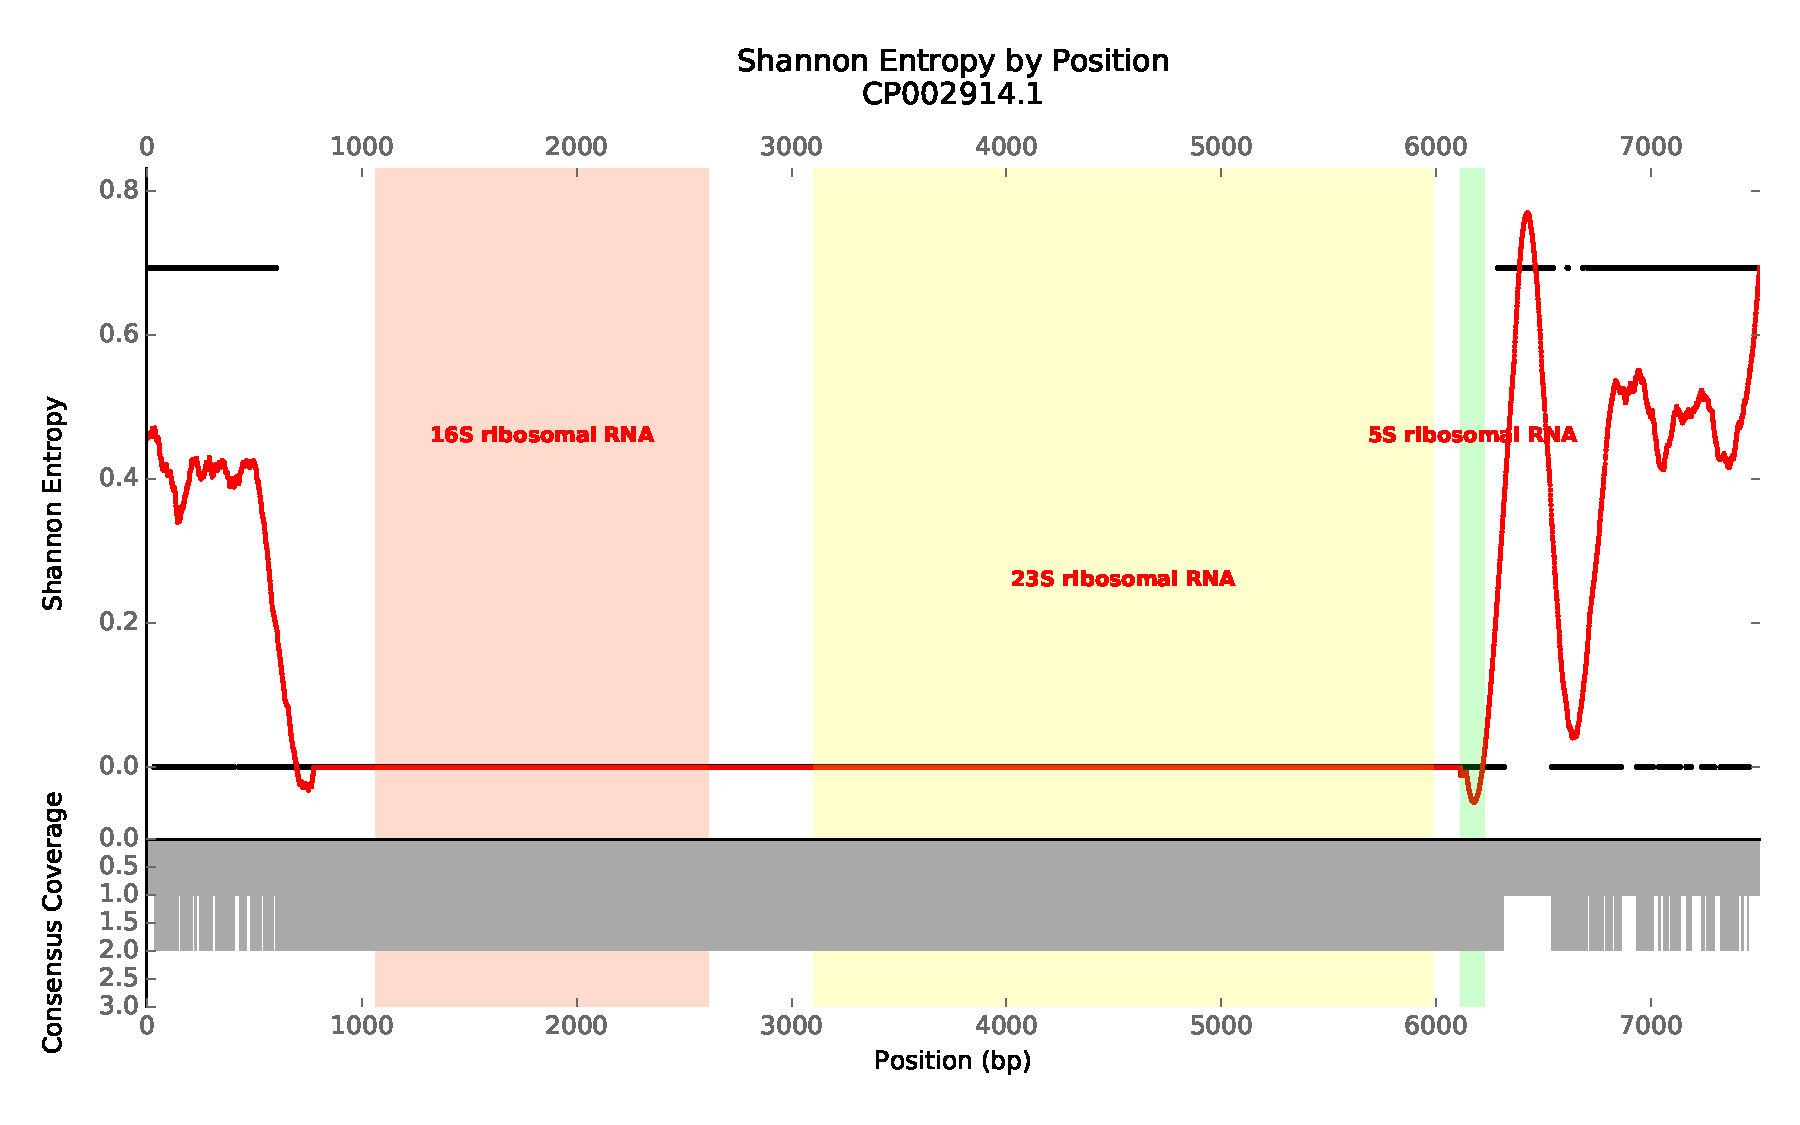
\includegraphics[width=0.95\textwidth]{gage_entropy_figures/CP002914.1_entropy_plot}
    \caption{\textit{X. axonopodis pv. Citrumelo} (CP002914.1)}
  \end{subfigure}
  \caption{riboScan.py,riboSelect.py, and riboSnag.py were run on all the genomes used as references for \textit{de fere novo} assemblies. Consensus alignment depth (grey bars) and Shannon entropy (black points, smoothed entropy as red line) for aligned rDNA regions.}
  \label{fig:ent_gage}

\end{figure}

\pagebreak


\section*{Extended Methods}

\subsection*{Reference Selection Recommendations}
Using a close reference sequence maximizes chances of a successful assembly. We have outlined two methods to select an appropriate reference for a given isolate: a robust method, and a quick method.

\subsubsection*{Method 1: Kraken}

Kraken\cite{Wood2014} is a kmer-based phylogeny tool that can be used to identify the strains present in a metagenomic dataset;  the installation and usage instructions can be found here: \href{https://ccb.jhu.edu/software/kraken/}{https://ccb.jhu.edu/software/kraken/}. After downloading and installing Kraken, along with the MiniKraken database from their website, Kraken can be run on an isolate's reads, generating the a taxonomy report.

The MiniKraken database was built from all the complete genomes from RefSeq, allowing the user to identify which strain in the database has the closest match to the sequenced isolate.

\subsubsection*{Method 2: Reads2Type and  cgFind}
Reads2Type\cite{Saputra2015} is also a kmer-based phylogeny tool, but it relies on a lightweight, prebuilt database of 55-mers from a set of reference strains. This allows the analysis to be performed in the web browser, and it does not require the user to upload the whole read files, allowing it to perform well when either speed or network access is limited.  It works by taking one read at a time from a file, generating 55-mers, and comparing to a prebuild database. If there is not enough resolution information to identify the isolate on that read alone, additional reads will be processed until a single taxonomy is achieved.  This method works best on trimmed reads. Instructions and the webserver can be found at \href{https://cge.cbs.dtu.dk/services/Reads2Type/}{https://cge.cbs.dtu.dk/services/Reads2Type/}

Now, given the genus and species from Reads2Type, users can make use of cgFind, our web tool developed to provide easy access to downloadable genomes based on the complete prokaryotic genomes found in NCBI. The tool can be found at \href{https://nickp60.github.io/cgfind}{https://nickp60.github.io/cgfind}.


\subsection*{Making the artificial test genome}
The artificial genome used for testing was constructed using the \texttt{makeToyGenome.sh} script included in the GitHub repository under the \textbf{\texttt{scripts}} directory. Briefly, the 7 rDNA regions from the \coli{Sakai} genome were extracted with 5kb flanking sequence upstream and downstream; these sequences were then concatenated end to end to form a single, \ttilde100kb sequence containing the 7 rDNAs as well as their flanking context.


\subsection*{Effect of reference sequence identity on riboSeed performance}
The following range of substitutions were introduced into a artificial genome using the \texttt{runDegenerate.sh} script (included in the GitHub repository under the \textbf{\texttt{scripts}} directory), which facilitates the following procedure: 0.0, 0.0025, 0.0050, 0.0075, 0.0100, 0.0150, 0.0200, 0.0250, 0.0500, 0.0750, 0.1000, 0.1250, 0.1500, 0.1750, 0.2000, 0.2250, 0.2500, 0.2750, 0.3000. An artificial test genome is constructed (see above), and reads simulated using pIRS (100bp, 300bp inserts, stdev 10, 30-fold coverage, built-in error profile).  Then, for each of a range of substitution frequencies, substitutions are introduced into the simulated genome, either just in the flanking regions or throughout. riboSeed is run on the reads using the mutated genome as the reference, and the results are evaluated with riboScore. This script was run 100 times, using a different random seed each time.  As pseudo random number generation may differ between operating systems, comparable but not identical results can be expected.

\section*{Performance on Archaeal Data}

We assessed the effectiveness of riboSeed with assembling archaeal genomes. Most (\ttilde55\%) archaeal genomes have only a single rDNA, and none has been observed to have more than four. As riboSeed requires a sequencing dataset and a reference genome, applicability was limited; of the 104 entries in \textit{rrn}DB with multiple rDNAs, only 7 had multiple entries at the species level. Among those, only 2 had publicly available short read data. We used riboSeed to re-assemble \textit{Methanosarcina barkeri Fusaro DSMZ804} (Illumina HiSeq 2000, 100bp paired-end reads) and \textit{Methanobacterium formicicum st. JCM10132} (DRR017790, Ion Torrent PGM, 89bp single-end reads). \textit{Methanobacterium formicicum st. BRM9} and \textit{Methanosarcina barkeri Fusaro DSMZ804} (SRR2064286) were the only ones that were suitable for riboSeed, meaning that there was publicly available short read data and that there is a related genome at the species level which is complete.

\textit{M. formicicum st. JCM10132} was sequenced on an Ion Torrent PGM, generating 106.5Mbp of single-end data. \textit{M formicicum BRM9} (CP006933.1) was used as a reference. While riboSeed with default parameters did not resolve any of the assembly gaps (final assembly kmers 21, 33, 55, and 77), re-running the final assembly with kmers of 21, 33, 55, 77, and 99 inexplicably resulted in closing 2 of 2 rDNA gaps. We are unsure why the addition of 99-mers improved assembly with 89-bp reads, but we are actively investigating this. This represents the first application of riboSeed to Ion Torrent data.


\textit{Methanosarcina barkeri Fusaro DSMZ804} was sequenced using an Illumina HiSeq2000 with 101bp paired-end reads, with an average fragment length of 400bp. We downsampled to use 5\% of the 19.4Gbp dataset with seqtk (\href{https://github.com/lh3/seqtk}{https://github.com/lh3/seqtk}). \textit{Methanosarcina barkeri str. Wiesmoor} (CP009526.1) was used as a reference. The resulting riboSeed assembly showed correct assembly of 3 of 3 rDNAs, while \textit{de novo} assemble failed to resolve any.

Taken together, we show that given appropriate datasets and parameters, archaeal datasets can be processed in the same manner used for bacteria.


\section*{Key Parameters}
\subsection*{\texttt{--ref\_as\_contig}}
The assembly that results from including riboSeed's ``long reads'' is sensitive to the manner in which they are incorporated into the \textit{de novo} assembly. Here, for our analyses, we used the SPAdes assembler \cite{Bankevich2012}, as it has built-in ways to include contigs (using the ``--trusted-contigs'' or ``--untrusted-contigs'') in FASTA format.  Other assemblers could be used, but most require long reads to have a quality score associate with them, preventing direct use of riboSeeds long reads.

As mentioned in the Methods section, riboSeed uses the reference rDNA region in the initial subassembly;  in subsequent subassemblies, the longest contig of the previous subsassembly is used.  These regions can be treated one of four ways using the \texttt{--ref\_as\_contig} argument: \texttt{trusted}, \texttt{untrusted}, \texttt{inferr}, or \texttt{ignore}.  Additionally, if the user is worried that the reference rDNA will too heavily influence the initial subassembly, they can enable the \texttt{--initial\_consensus} flag to use a mapping consensus assembly instead of the de Bruijn graph based assembly from SPAdes.

The default manner in which rDNA regions (either from the reference or from the previous iteration's subassembly) behaviour is to infer (\texttt{--ref\_as\_contig infer}): if the percent of reads mapping to  the (whole) reference sequence  is over 80\%, than the rDNA region will be included as a trusted contig.  If below 80\%, the reads will be treated as untrusted.

If a user wishes to have the subassemblies only using the reads (true \textit{de novo} assembly), they can use the \texttt{ignore} option.  We only recommend this with very close references.

Further, if the user wishes to explicity define the behaviour, \texttt{trusted} or \texttt{untrusted} can be provided to the \texttt{--ref\_as\_contig} argument.

\subsection*{\texttt{--score\_min}}
By default, the accepted alignment score for BWA mapping is $\frac{1}{2}$ the read length.  If needed, this can be increased for greater stringency when dealing with more divergent references, or decreased to include more reads, which may be adventageous when assembling a low coverage dataset.

\section*{Excluding GAGE-B HiSeq \textit{B. cereus}}

\begin{figure}[H]
  \centering
  \begin{subfigure}[b]{.5\textwidth}
    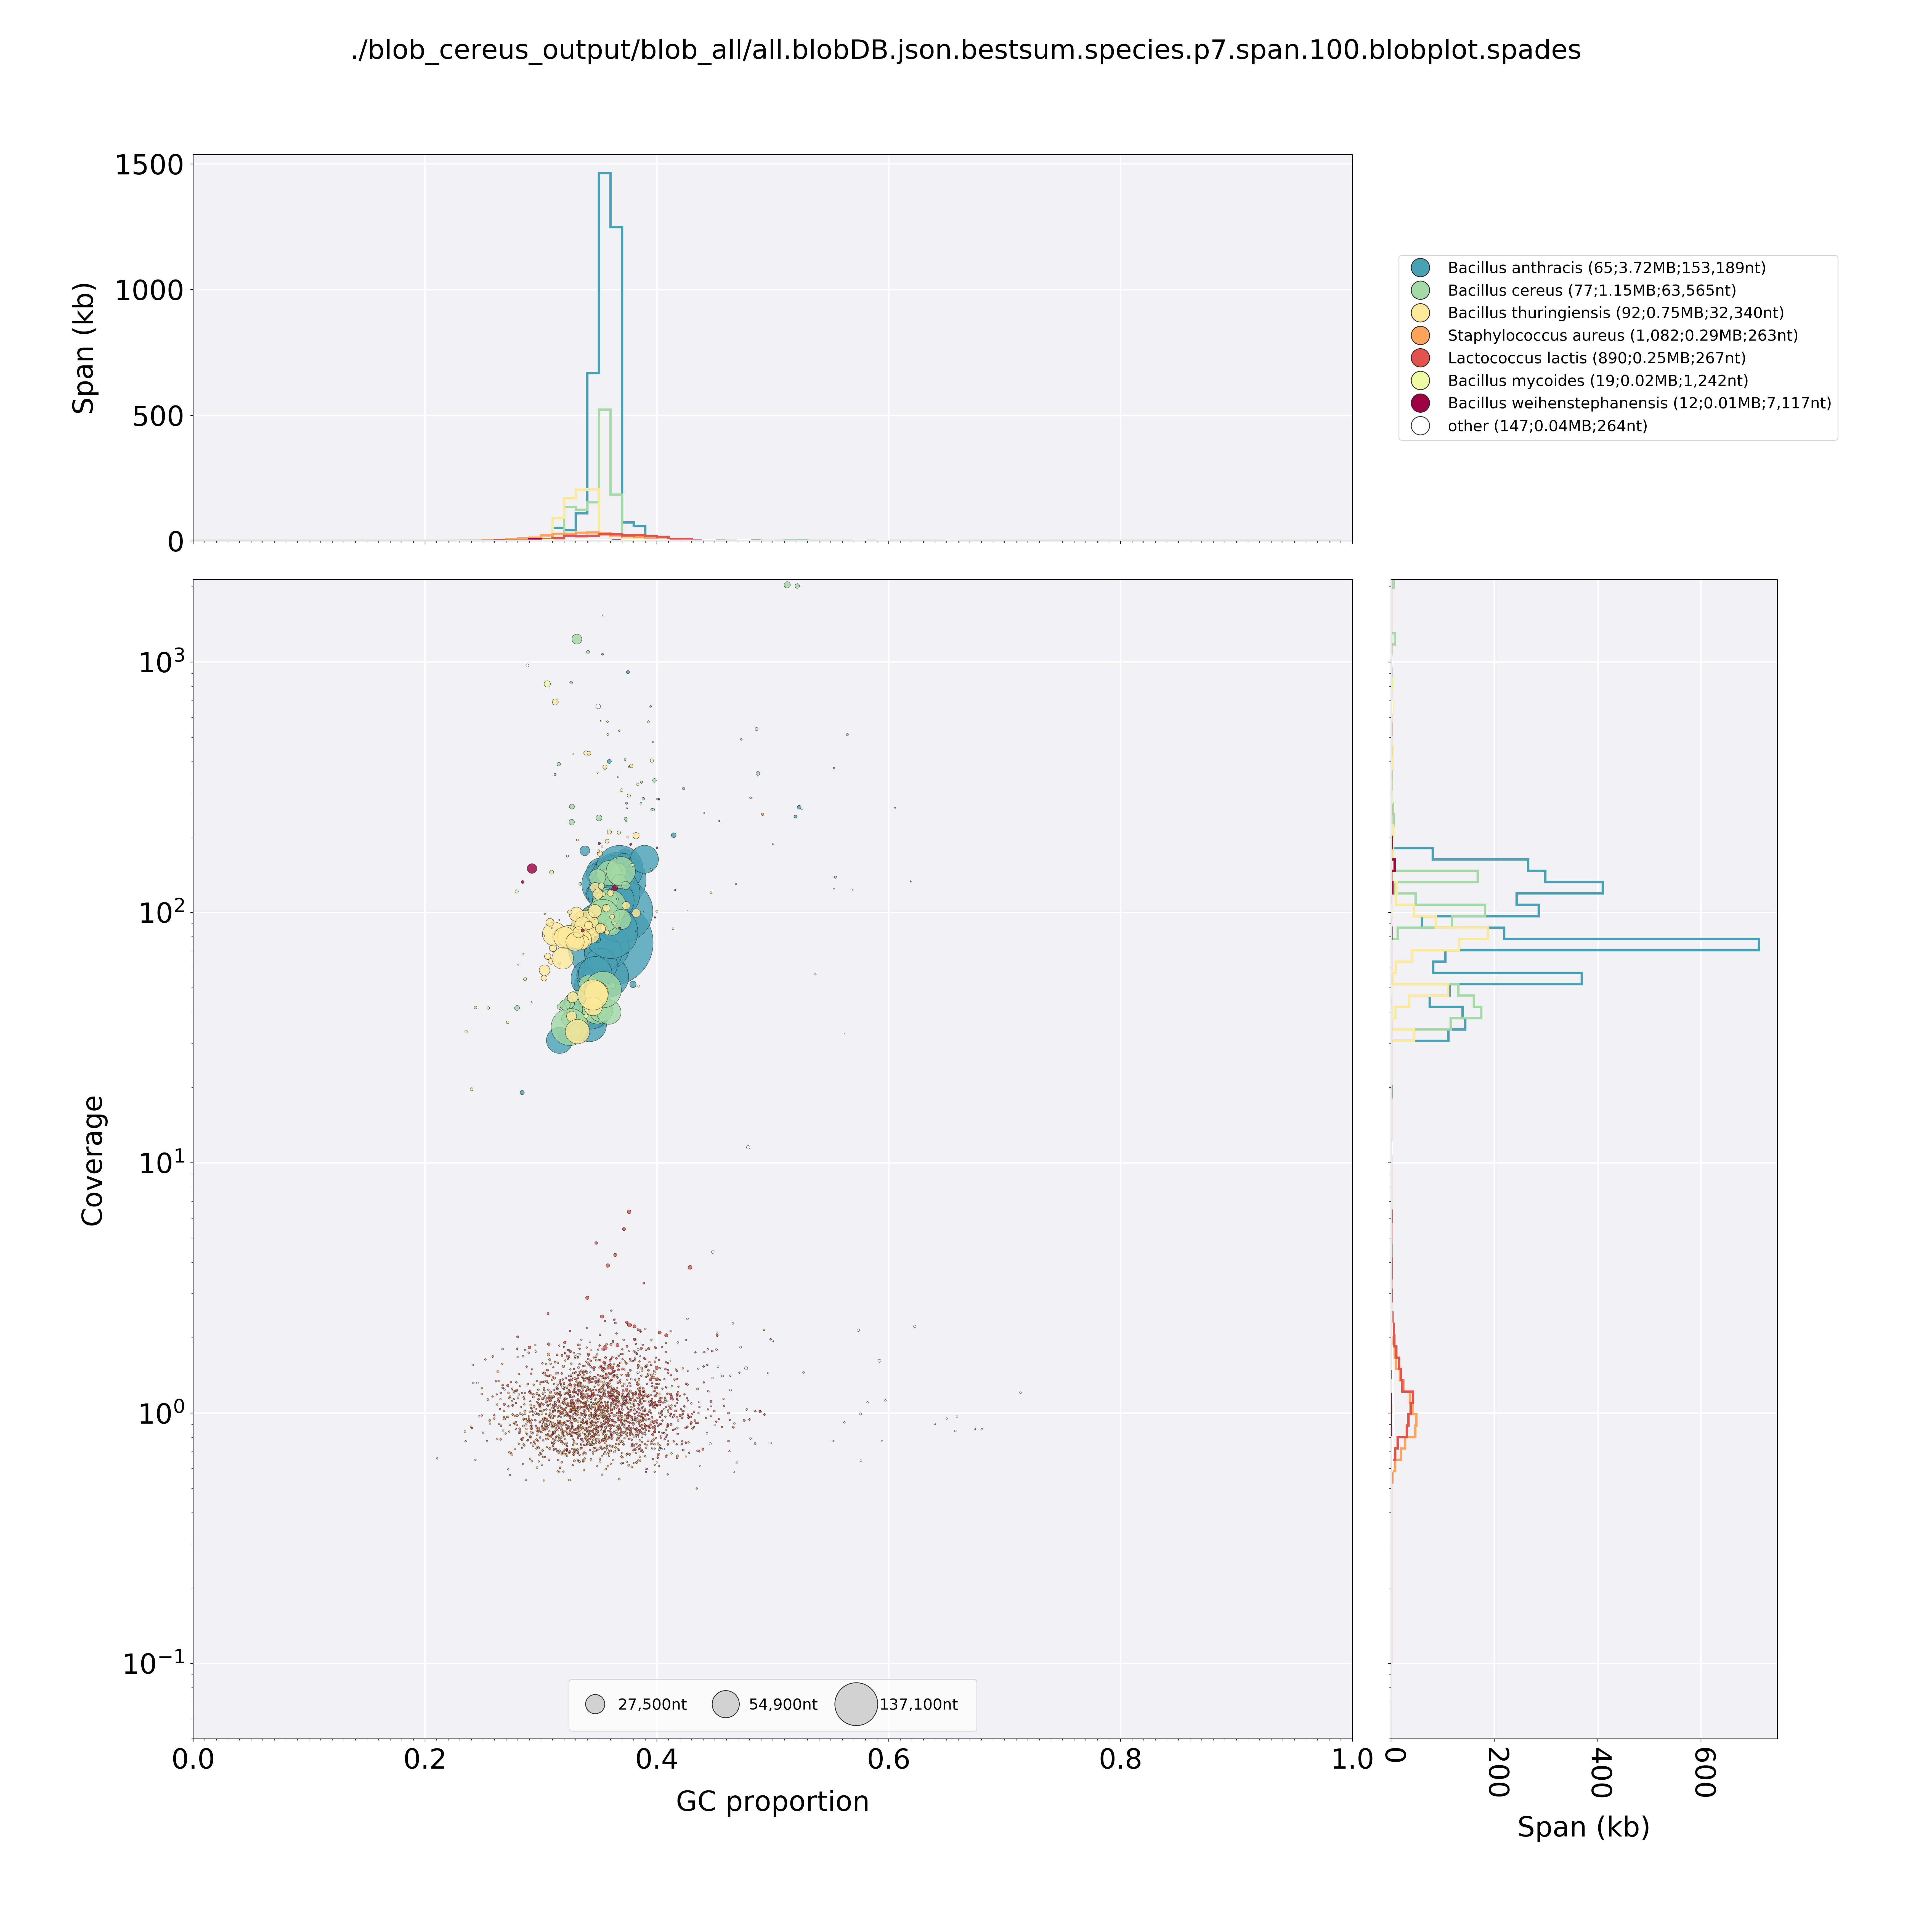
\includegraphics[width=.95\textwidth]{all.blobDB.json.bestsum.species.p7.span.100.blobplot.spades.png}
    \caption{All reads}
  \end{subfigure}
  \begin{subfigure}[b]{.5\textwidth}
    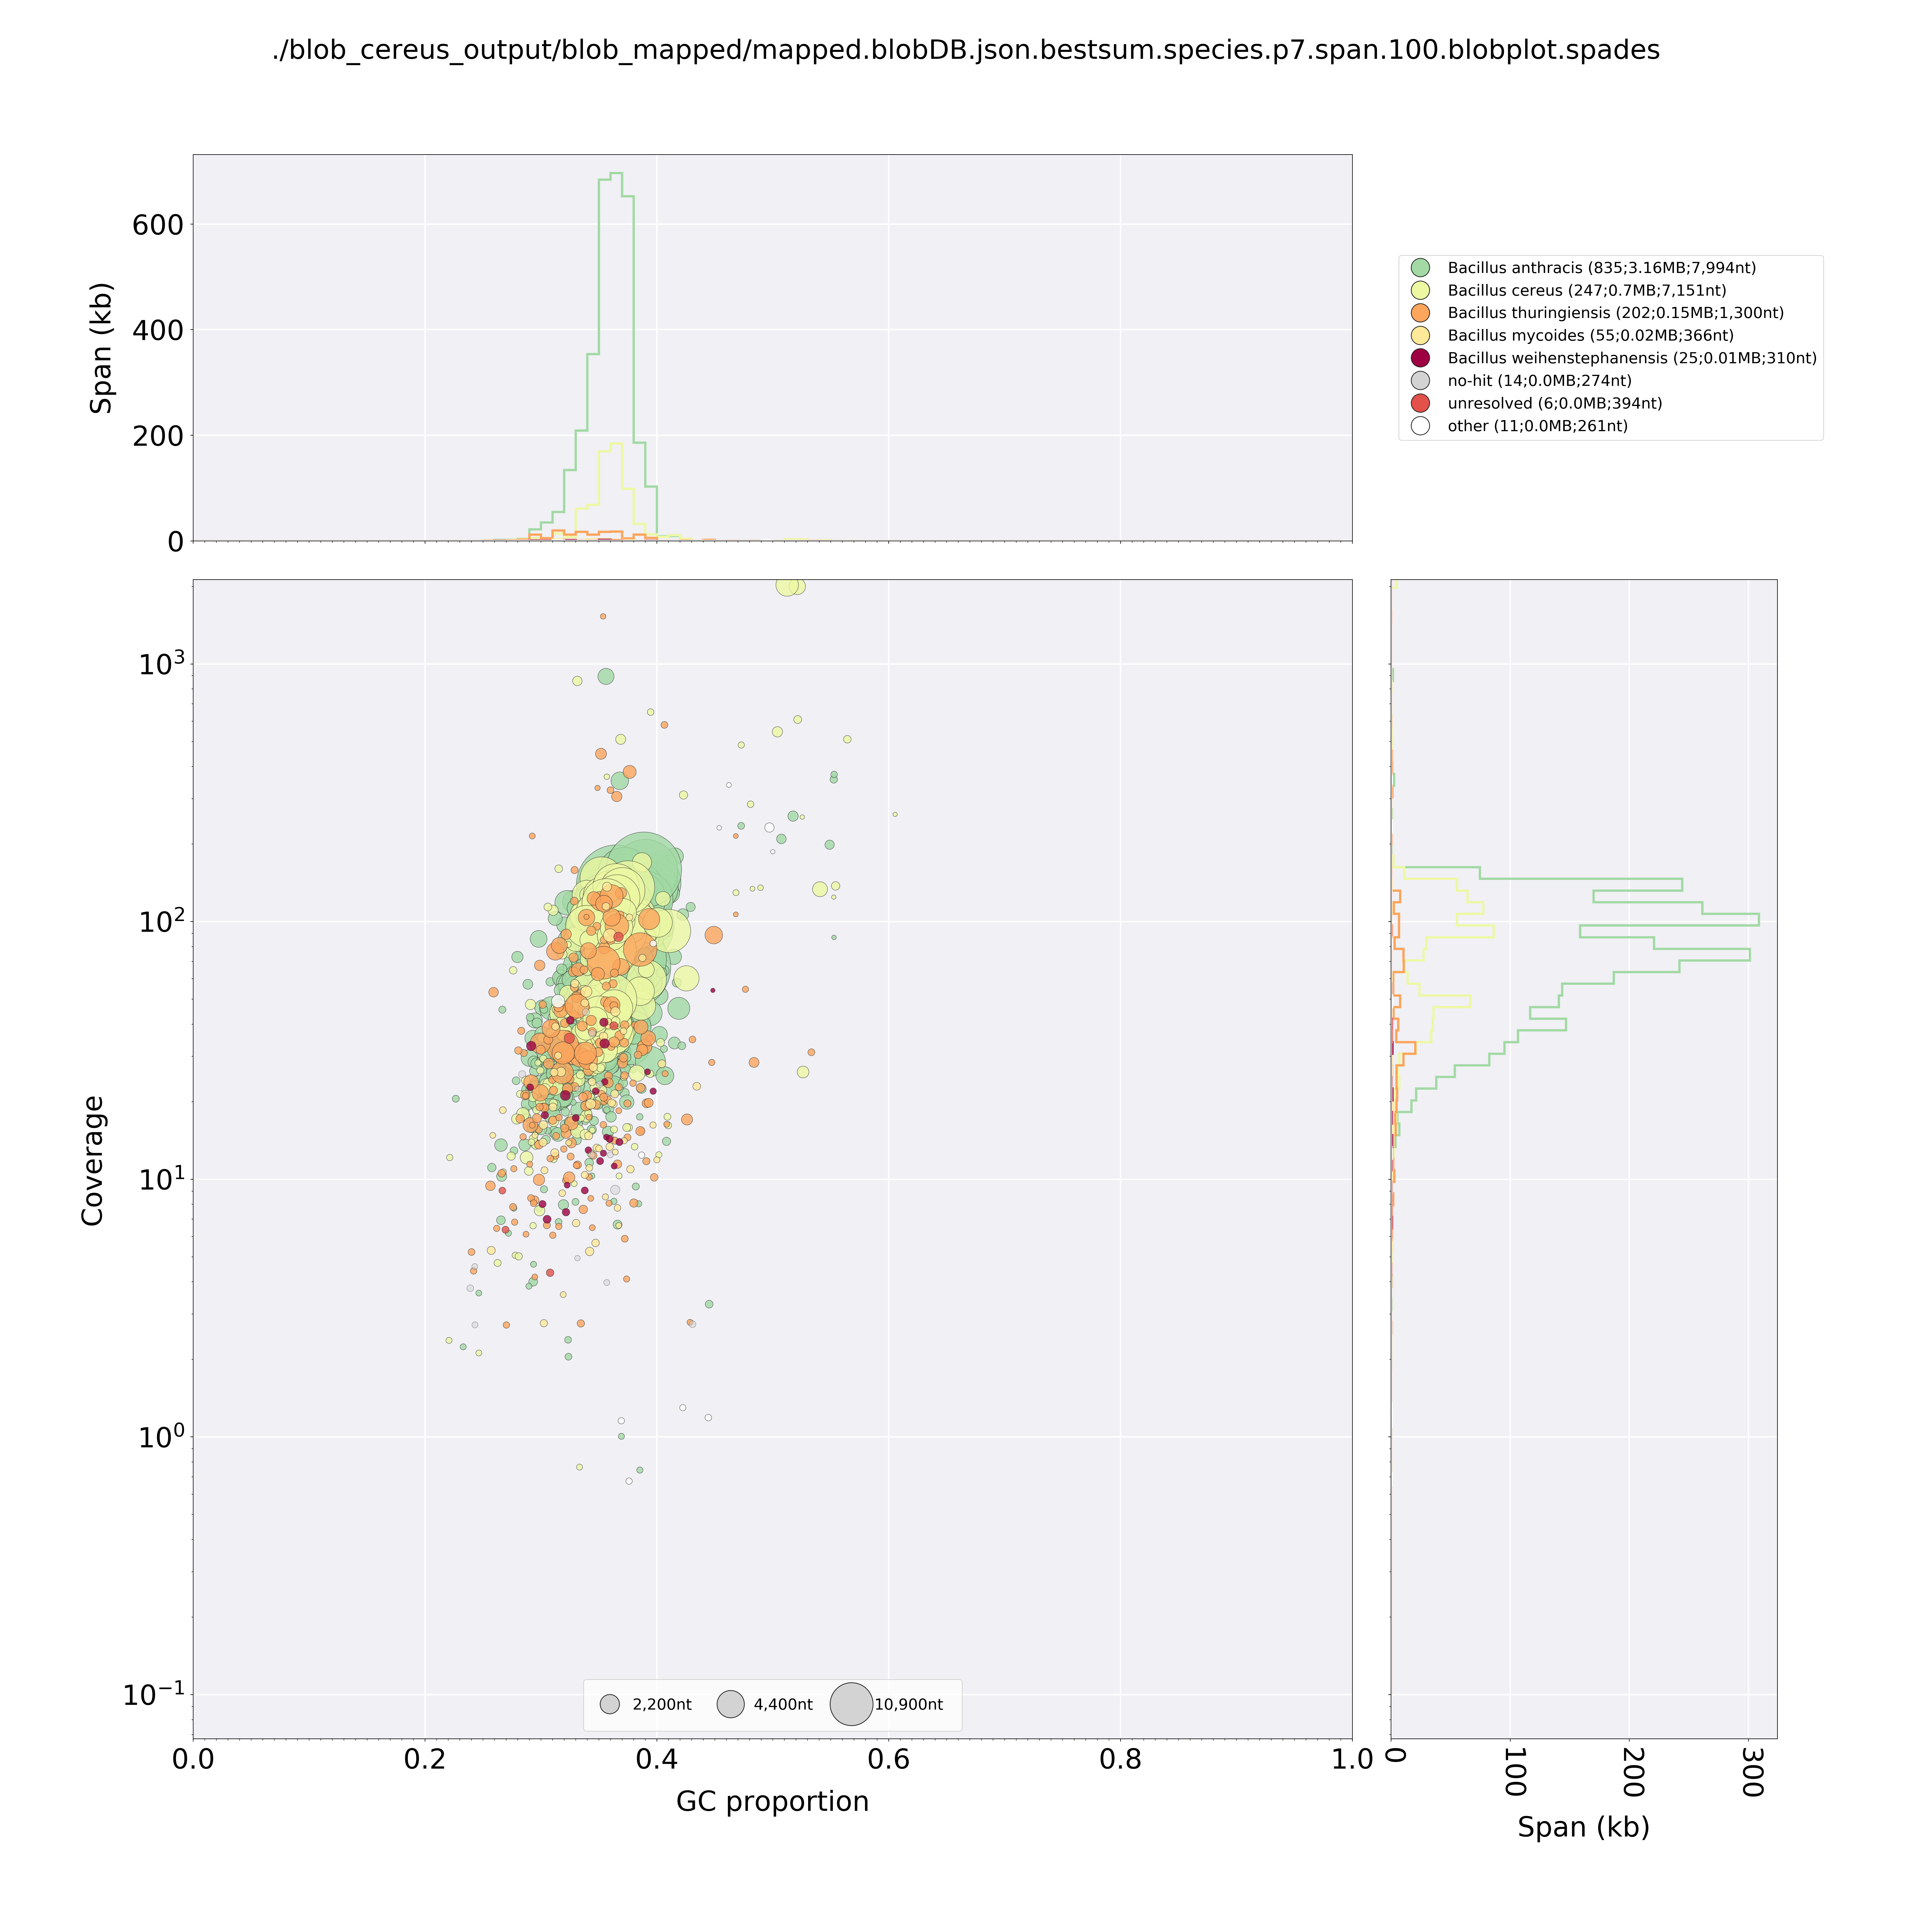
\includegraphics[width=.95\textwidth]{mapped.blobDB.json.bestsum.species.p7.span.100.blobplot.spades.png}
    \caption{Reads aligning to reference}
  \end{subfigure}
  \begin{subfigure}[b]{.5\textwidth}
    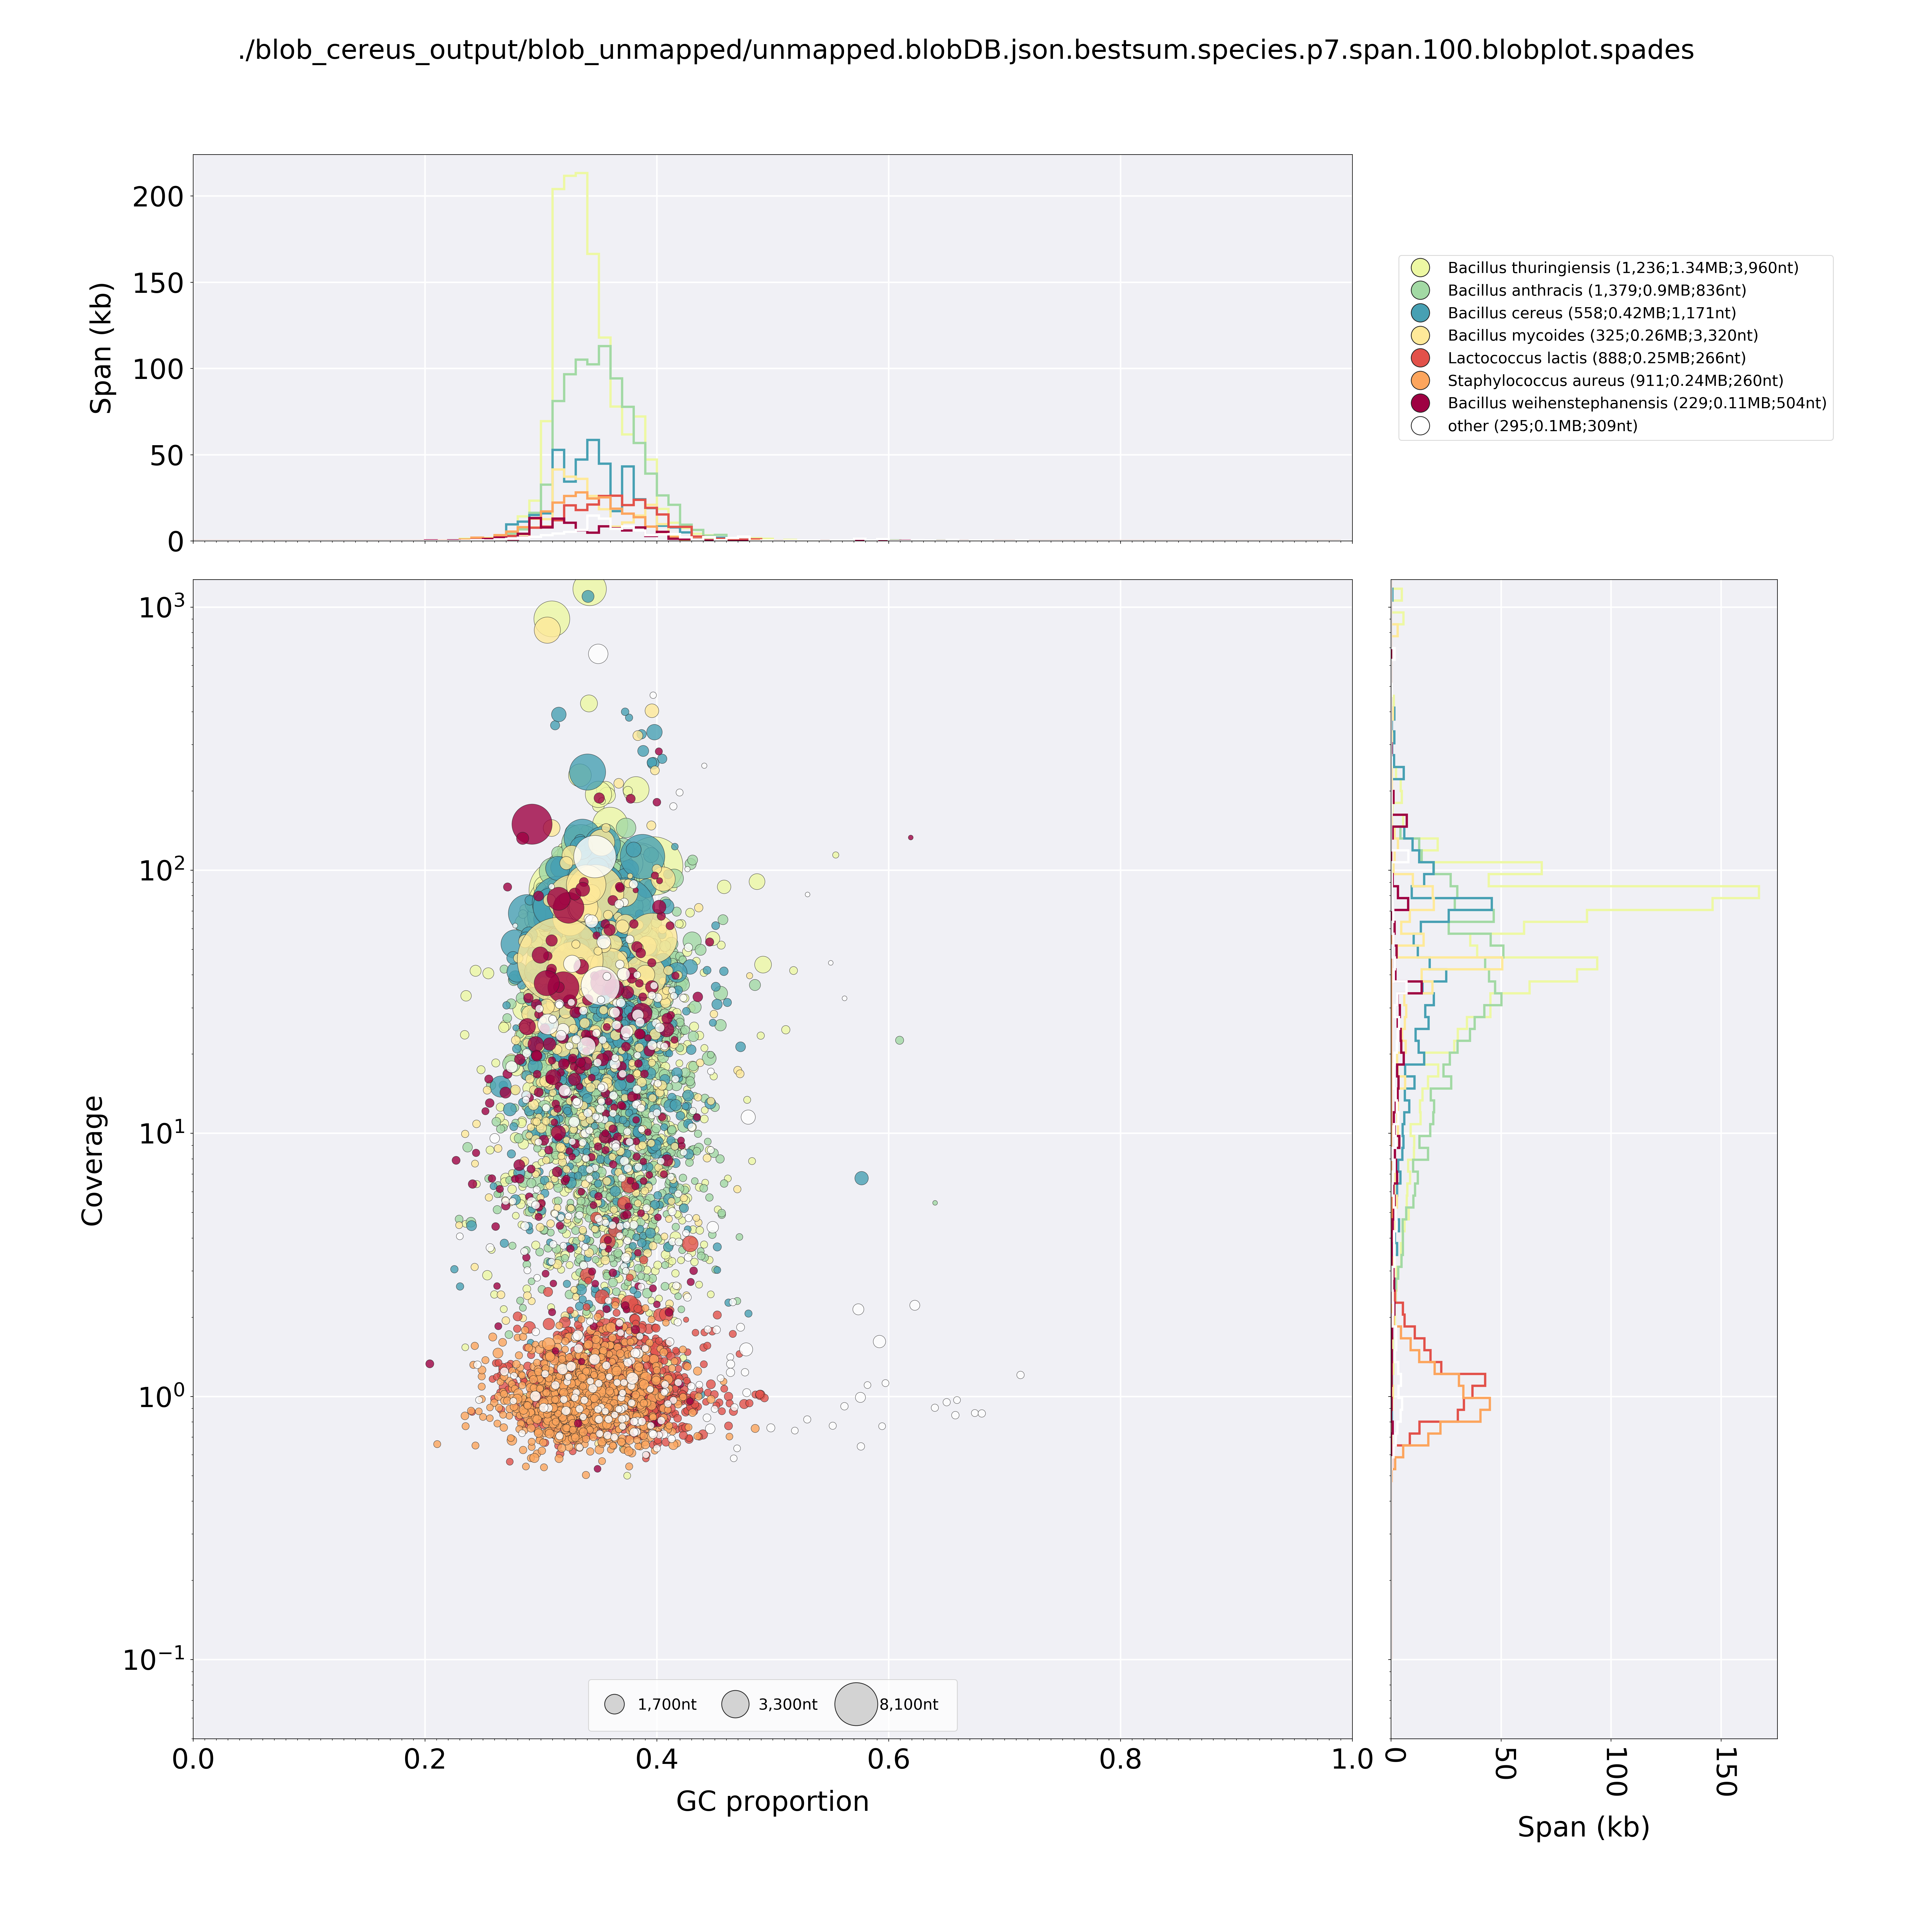
\includegraphics[width=.95\textwidth]{unmapped.blobDB.json.bestsum.species.p7.span.100.blobplot.spades.png}
    \caption{Reads failing to align to reference}
  \end{subfigure}
  \caption{Assessing contamination in the GAGE-B HiSeq \textit{B. cereus} dataset with blobtools. Reads were assembled with metaSPAdes, taxanomically assigned with BLASTn against the nt database, and plotted with blobtools.  (A) shows the whole dataset, while (B) and (C) shows the portion of the reads aligning to the \textit{B. cereus} ATCC 10987 reference and those failing to align, respectively.}
  \label{fig:contamination_all}
\end{figure}

The GAGE-B paper \cite{Magoc2013} notes that the \textit{B. cereus} HiSeq dataset proved particularly difficult to assemble. After noticing this irregularity, we re-assembled the trimmed reads downloaded from the GAGE-B website with metaSPAdes\cite{Nurk2017}  using default parameters.  Then, blastn was used to search the resulting contigs against NCBI's nt database (May, 2017) to get a list of hits according to the blobtools <cite> specifications. Blobtools was then used to plot the hit coverage, taxonomy, and GC-content of the contigs.  This revealed what appears to be a contamination. \ref{fig:contamination_all}A. As the GC content of the contaminating organisms did not differ from \textit{B. cereus}, we believe that many tools that use GC-skew to detect contamination would not have detected the problem with this dataset.


To further show the contamination, we split reads into those read pairs mapping to the \textit{B. cereus} ATCC 10987 reference genome and those unmapped.  BWA MEM\cite{Li2013} was used to map the 12039737 reads to the reference genome;  samtools was used to separate the 7500534 reads (62\%) that mapped from the 3984200 reads (33\%) that failed to map with default parameters\footnote{The remaining \ttilde5 percent are those pairs where only one read aligned to the reference; these were ignored for this analysis.}.Each of these sets of reads was then assembled, BLASTed against the nt database, and plotted with blobtools \ref{fig:contamination_all}B and C.


Further, MaxBin\cite{Wu2014}, Kraken, and MBBC\cite{Wang2011} also supported the hypothesis that the sample is contaminated with approximately one third of reads originating from a non-\textit{B. cereus} strain.


\thoughtbr
\newpage

\begin{table}[]
  \centering
  \caption{Hits resulting from searching the SRA database for various sequencing technologies as of January, 2017}
  \label{table:searchterms}
  \begin{tabular}{lrr}
    \toprule
    Search term & Hits & Percentage \\
    \midrule
    illumina & 2242225 & 94.27 \\
    pacbio & 21131 & 0.89 \\
    ion & 30560 & 1.28 \\
    roche & 42445 & 1.78 \\
    oxford & 12301 & 0.52 \\
    solid & 29791 & 1.25 \\
    \arrayrulecolor{lgray}\hline
    Total & 2378453 & 100\\
    \arrayrulecolor{black}
    \bottomrule
\end{tabular}
\end{table}

%%%%%%%%%%%%%%%%%%%%%%%%%%%%%%%%%%%%%%%%%%%%%%%%%%%%%%%%%%%%%%%%%%%%%%%
\begin{table}[!h]
\centering
\caption{Accessions for 25 \textit{E. coli} genomes}
\label{table:accessions}
\begin{tabular}{l}
  \toprule

  GCA\_000005845.2\_ASM584v2                    \\
  GCA\_000019385.1\_ASM1938v1                   \\
  GCA\_000026245.1\_ASM2624v1                   \\
  GCA\_000026345.1\_ASM2634v1                   \\
  GCA\_000026545.1\_ASM2654v1                   \\
  GCA\_000146735.1\_ASM14673v1                  \\
  GCA\_000257275.1\_ASM25727v1                  \\
  GCA\_000520055.1\_ASM52005v1                  \\
  GCA\_000732965.1\_ASM73296v1                  \\
  GCA\_001007915.1\_ASM100791v1                 \\
  GCA\_001442495.1\_ASM144249v1                 \\
  GCA\_001469815.1\_ASM146981v1                 \\
  GCA\_001660565.1\_ASM166056v1                 \\
  GCA\_001660585.1\_ASM166058v1                 \\
  GCA\_001753565.1\_ASM175356v1                 \\
  GCA\_001888075.1\_ASM188807v1                 \\
  GCA\_001901025.1\_ASM190102v1                 \\
  GCA\_001936315.1\_ASM193631v1                 \\
  GCA\_002056065.1\_ASM205606v1                 \\
  GCA\_002078295.1\_ASM207829v1                 \\
  GCA\_002156825.1\_ASM215682v1                 \\
  GCA\_002163935.1\_ASM216393v1                 \\
  GCA\_002192275.1\_ASM219227v1                 \\
  GCA\_002220265.1\_ASM222026v1                 \\
  GCA\_900096795.1\_Ecoli\_AG100\_Sample3\_Doxycycline\_Assembly \\
  \bottomrule
  {\tiny   All available at \texttt{ftp://ftp.ncbi.nlm.nih.gov/genomes/all/GCA/}}

\end{tabular}
\end{table}
%%%%%%%%%%%%%%%%%%%%%%%%%%%%%%%%%%%%%%%%%%%%%%%%%%%%%%%%%%%%%%%%%%%%%%%



\begin{table}[]
\centering
\caption{Strain names and accessions for reference genomes used in this study}
\label{table:strainlist}
\begin{tabular}{ll}
  \toprule
  Strain Name & Accession \\
  \midrule
  \textit{E. coli MG1655} & NC\_000913.3 \\
  \textit{A. hydrophila ATCC 7966} & NC\_008570.1 \\
  \textit{B. cereus ATCC 10987} & AE017194.1 \\
  \textit{B. cereus NC7401} & NC\_016771.1 \\
  \textit{B. fragilis 638R} & FQ312004.1 \\
  \textit{R. sphaeroides ATCC 17029} & NC\_009049.1, NC\_009050.1 \\
  \textit{S. aureus TCH1516} & NC\_010079.1 \\
  % \textit{S. aureus NCTC 8325} & NC\_007795.1 \\
  % \textit{S. aureus FDA209P} & AP014942.1 \\
  \textit{S. aureus MRSA252} & BX571856.1 \\
  \textit{V. cholerae El Tor str. N16961} & NC\_002505.1, NC\_002506.1 \\
  \textit{X. axonopodis pv. Citrumelo} & CP002914.1 \\
  \textit{P. aeruginosa BAMCPA07-48} & CP015377.1 \\
  \textit{P. aeruginosa ATCC 15692} & NZ\_CP017149.1\\
  \bottomrule

\end{tabular}
\end{table}

\begin{table}[]
  \centering
  \caption{Software Versions}
  \label{table:software}
  \begin{tabular}{ll}
    \toprule
    Tool & Version \\
    \midrule
    Mauve & 2015-02-13 build 0 \\
    BLAST+ & 2.2.28+ \\
    Barrnap & 0.8 \\
    BWA & 0.7.8-r455 \\
    samtools & 1.4.1 \\
    MAFFT & v7.310 \\
    SPAdes & v3.9.0 \\
    QUAST & 4.4 \\
    bedtools & 2.17.0 \\
    EMBOSS & 6.5.7 \\
    pIRS & 2.0.2\\
    seqtk & 1.2-r94\\
    Parsnp & v1.2 \\
    \bottomrule
  \end{tabular}
\end{table}

\begin{table}[]
\centering
\caption{QUAST results of \textit{P. aeruginosa} BAMCPA07-48 assemblies comparing \textit{de fere novo} assembly, \textit{de novo} assembly, and reference-based assembly (where the \textit{P. aeruginosa} ATCC 15692 reference is included in the \textit{de novo} assembly as a trusted contig).  Blue and red highlight the best and worst results, respectively.  riboSeed's \textit{de fere novo} assembly either outperforms or performs comparably to \textit{de novo} assembly in all categories.  Using the reference as a trusted contig results in longer assemblies but with a much higher rate of missmatches, indels, and missasemblies.}
\label{table:full_ref_compare}
\begin{tabular}{llll}
\textbf{Genome statistics} & \textbf{\textit{de fere novo}} & \textbf{\textit{de novo}} & \textbf{reference-based} \\
Genome fraction (\%) & \cellcolor[HTML]{CDCDF9}98.106 & \cellcolor[HTML]{FBDADA}97.868 & 98 \\
Duplication ratio & 1.001 & 1.001 & \cellcolor[HTML]{FBDADA}1.017 \\
Largest alignment & 630503 & \cellcolor[HTML]{FBDADA}402463 & \cellcolor[HTML]{CDCDF9}757685 \\
Total aligned length & 6893293 & \cellcolor[HTML]{FBDADA}6876715 & \cellcolor[HTML]{CDCDF9}6993532 \\
NGA50 & 176510 & 176510 & \cellcolor[HTML]{FBDADA}135376 \\
LGA50 & \cellcolor[HTML]{CDCDF9}12 & 13 & \cellcolor[HTML]{FBDADA}14 \\
\textbf{Misassemblies} &  &  &  \\
\# misassemblies & 2 & 2 & \cellcolor[HTML]{FBDADA}9 \\
Misassembled contigs length & 212498 & 212498 & \cellcolor[HTML]{FBDADA}2347560 \\
\textbf{Mismatches} &  &  &  \\
\# mismatches per 100 kbp & 1.89 & \cellcolor[HTML]{CDCDF9}1.69 & \cellcolor[HTML]{FBDADA}11.66 \\
\# indels per 100 kbp & 2.48 & \cellcolor[HTML]{CDCDF9}2.44 & \cellcolor[HTML]{FBDADA}2.94 \\
\# N's per 100 kbp & 0 & 0 & 0 \\
\textbf{Statistics without reference} &  &  &  \\
\# contigs & \cellcolor[HTML]{CDCDF9}154 & 159 & 388 \\
Largest contig & 630503 & \cellcolor[HTML]{FBDADA}402463 & \cellcolor[HTML]{CDCDF9}1103106 \\
Total length & 6893293 & \cellcolor[HTML]{FBDADA}6876715 & \cellcolor[HTML]{CDCDF9}7237564 \\
Total length (\textgreater= 1000 bp) & 6865091 & \cellcolor[HTML]{FBDADA}6848513 & \cellcolor[HTML]{CDCDF9}7130244 \\
Total length (\textgreater= 10000 bp) & \cellcolor[HTML]{CDCDF9}6687664 & 6663031 & \cellcolor[HTML]{FBDADA}6617370 \\
Total length (\textgreater= 50000 bp) & \cellcolor[HTML]{CDCDF9}6242010 & 6168232 & \cellcolor[HTML]{FBDADA}5534330
\end{tabular}
\end{table}


%%%%%%%%%%%%%%%%%%%%%%%%%%%%%%%%%%%%%%%%%%%%%%%%%%%%
\pagebreak
%%%%%%%%%%%%%%%%%%%%%%%%%%%%%%%%%%%%%%%%%%%%%%%%
\bibliographystyle{unsrt}
\bibliography{/home/nicholas/GitHub/riboSeed/Waters_et_al_2017/ms/riboSeed_refs}

\end{document}
